\documentclass{beamer}

\usepackage{subfigure}
\usepackage{graphicx}
\usepackage{sidecap}
\usepackage{caption}
%\usepackage{subcaption}
\captionsetup{compatibility=false}
\usepackage{appendixnumberbeamer}
\usepackage{amsmath}
% --
\usepackage{multirow}
\usepackage{xcolor}
\usepackage{setspace}
\usepackage{hyperref}
\usepackage{anyfontsize}

\beamertemplatenavigationsymbolsempty
\setbeamertemplate{footline}

\newenvironment{itemise} {\begin{itemize} \setlength{\itemsep}{0.2cm}} {\end{itemize}}
\usepackage[labelformat=empty]{caption}
\setbeamertemplate{sections/subsections in toc}[square]

%% COLORS
\definecolor{Gray}{gray}{0.9}
\definecolor{dblue}{rgb}{0.132,0.1,0.27}
\definecolor{mint}{cmyk}{1.0, 0.2, 0.6, 0.05}
\definecolor{ant}{cmyk}{0.5, 0.1, 0.0, 0.45}
\definecolor{lgray}{cmyk}{0.12, 0.0, 0.0, 0.17}
\definecolor{lred}{cmyk}{0.0, 0.9, 0.7, 0.0}


\usepackage{etoolbox}% http://ctan.org/pkg/etoolbox 
\usepackage{booktabs}

\newenvironment{literatur}{%
  \parskip2pt \parindent0pt \raggedright
  \def\lititem{\hangindent=0.5cm \hangafter1}}{%
  \par\ignorespaces}

\newcommand{\tb}[1]{{\color{blue}{\textbf{#1}}}}
\newcommand{\tm}[1]{{\color{mint}{\textbf{#1}}}}
\newcommand{\tr}[1]{{\color{red}{\textbf{#1}}}}
% Ilya: packages

\usepackage{tikz}
\usepackage{lmodern}
\usepackage{enumitem}

% Ilya: my commands

\newenvironment{mytemize}
{\vfill\itemize[nolistsep,itemsep=\fill,label=\color{blue}{$\triangleright$}]}
  {\enditemize}


\newenvironment{mynumerate}
{\vfill\enumerate[nolistsep,itemsep=\fill,label=\arabic*.]}
  {\endenumerate}

\newcommand{\hitem}[1]{
  {\color{blue}{$\triangleright$}} 
  {#1} 
  {\hfill}
}

\setlist[itemize]{label= \color{blue}{$\triangleright$}}
\setlist[enumerate]{label = \arabic*.}

\newcommand{\rarr}{$\Rightarrow$\ }



%\href{<Ziel>}{<Eingefasster Text>} 

%\logo{\includegraphics[height=0.7cm]{BdFlogo.eps}\hspace{300pt}\vspace{-5pt}}
%\logo{\includegraphics[height=0.8cm]{BdFlogo.eps}}
%\logo{\pgfputat{\pgfxy(-6.2,-0.5)}{\pgfbox[center,base]{\includegraphics[height=0.8cm]{BdFlogo.eps}}}}

%------------------------------------------------------------------------------------
% TITLE
%------------------------------------------------------------------------------------
\title[PSME]{Macroeconomics\\ Lecture 2 --- AD-AS, Introduction to Dynamics}
\author[I. Eryzhenskiy]{Ilya Eryzhenskiy}
\institute[BdF]{PSME Panth\'{e}on-Sorbonne Master in Economics}
\date[PSME macro]{Fall 2023}


%---BEGIN------------------------------------------------------------------------------
\begin{document}
%---BEGIN------------------------------------------------------------------------------
\begin{frame}
\maketitle
\end{frame}
%---FRAME------------------------------------------------------------------------------
%---FRAME------------------------------------------------------------------------------
%---FRAME------------------------------------------------------------------------------
\begin{frame}{Lecture overview}

\begin{mytemize}
\item So far, very short run \rarr prices fixed \rarr no modelling of \textit{inflation dynamics}
\item This lecture:
\begin{mytemize}
\item \textbf{Long run}: flexible prices \rarr \tb{Monetary Neutrality}
\item \textbf{Medium run}: prices adjust in response to excess demand and supply of goods, but not all markets clear fully.
\item[\rarr] \tb{Phillips curve} and \tb{AS} curve, the two closely related
\end{mytemize}
\end{mytemize}
\end{frame}
%---FRAME------------------------------------------------------------------------------
\section{Phillips curve}
\subsection{General Equilibrium with Flexible Prices}
\begin{frame}{Supply-determined output in the long run}

\begin{columns}

\column{0.65\linewidth}
\begin{itemize}
\item What determines output in the \textbf{long run (on the trend)}?
\item Simplistic production theory:
\begin{itemize}
\item Only labor ($L$) used for production
\item $L$'s \tb{marginal product} $=$ \tb{real wage} \rarr equilibrium $\bar L$, output $\bar Y$
\end{itemize}
\item What about demand? 
  \begin{itemize}
	\item In the medium run, \textbf{demand adjusts to supply} via \tb{real wage}
  \end{itemize}
\end{itemize}

% COLUMN(2)
\column{0.35\linewidth}

\centering
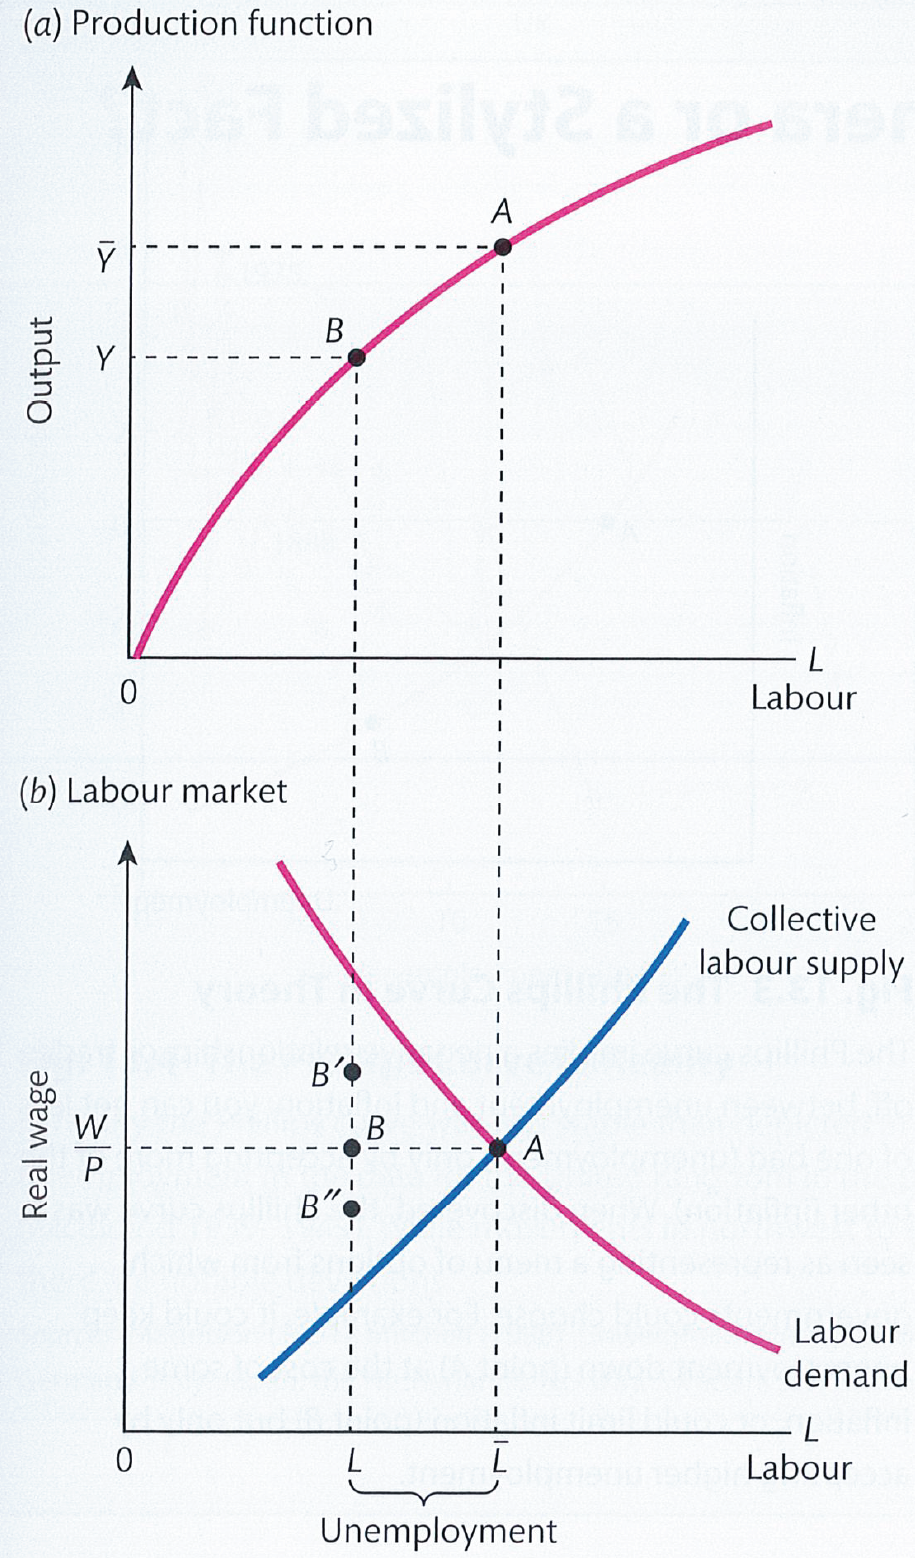
\includegraphics[clip,width=1.1\columnwidth]{FIGURES/8_LongRun}
%\vspace{-2mm}

\begin{minipage}{1.0\columnwidth}
\tiny	
%	\textbf{Note.} The Figure shows the average behaviour of variables around cyclical peaks in eight countries.\\
\textbf{Source.} Burda and Wyplosz (2017), Figure 13.2.\\
\end{minipage}
	
\end{columns} 	       

\end{frame}

\begin{frame}{Money and inflation in long run}

  Start with the \tb{Cambridge equation} (Quantity Theory of money):
\begin{align*}
M &= kPY \\
\Leftrightarrow \quad P &= \frac{M}{kY}
\end{align*}
assuming \textit{money velocity} $k$ constant, logarithms of both sides and a total differential:
\begin{align*}
\ln P &= \ln M - \ln k - \ln Y \\ 
\text{total differential:} \quad  \frac{d P}{P} &= \underbrace{\frac{d M}{M}}_{\equiv \mu} - \underbrace{\frac{d k}{k}}_{=0} - \underbrace{\frac{d Y}{Y}}_{\equiv g} \\ 
\Leftrightarrow \pi &=  \mu - g 
\end{align*}

\end{frame}
%---FRAME------------------------------------------------------------------------------
\begin{frame}{Monetary policy, interest in the long run}

  The long-run  inflation is the inflation target in the Taylor rule: $\bar \pi = \mu - g$. Target depends on:
  \begin{mynumerate}
	\item Money growth rate $\mu$, a policy variable
	\item Trend growth rate $g$ determined (mostly) by technology and demographics
  \end{mynumerate}
  $\pi = \bar \pi, Y = \bar Y$ in the long run, so from the TR equation:
\begin{align*}
i = \bar{i}+a (\pi - \bar{\pi}) + b \left(\frac{Y-\bar{Y}}{\bar{Y}} \right) = \bar i
\end{align*}
\vfill
Nominal interest at its long-run target --- the \tb{natural interest rate}. Real interest rate: 
\begin{align*}
\bar r = \bar i - \bar \pi = \bar i - \mu + g
\end{align*}
Technology and demographics affect the real interest rate: it is high in an economy with faster trend growth.
\end{frame}

\begin{frame}{Real natural interest estimates in developed economies}

\begin{mytemize}
\item $\bar r$ has a common tendency between countries; very low or negative levels in the 2010s 
\end{mytemize}
\begin{center}
%{\small
%\tb{Figure.} Frequency of price increases and price decreases \\
%}

\vspace{-2mm}
\begin{figure}[h!]
%\caption{Figure. Capital share US, 1946-2018
	%\subfigure{\includegraphics<1>[trim=80 60 100 70,clip,width=0.75\textwidth]{FIGURES/3_Autarky}
	%}
	\subfigure{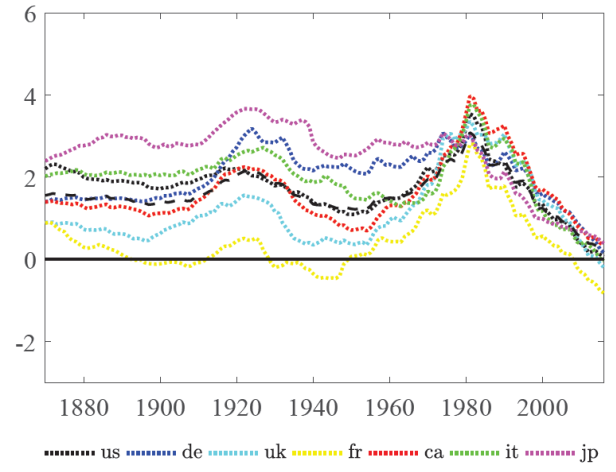
\includegraphics[trim=0 0 0 0,clip,width=0.6\textwidth]{FIGURES/6_ChangesRstar}
	}      
	%\subfigure{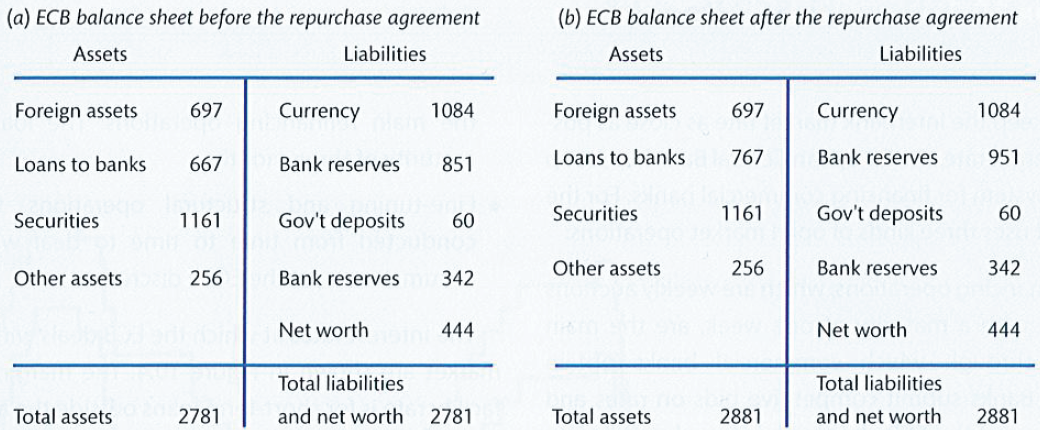
\includegraphics[trim=0 00 0 00,clip,width=0.6\textwidth]{FIGURES/5_CB_balance_sheet_OMO}
	%} 
	
%	\label{fig:GPD} 
	%[trim=left bottom right top
\end{figure}
%\vspace{-2mm}

\begin{minipage}{1.0\columnwidth}
\tiny	
\textbf{Note.} Estimates from a Bayesian factor model with country-specific and global trend for the real natural rate of interest, $r^*_i$.
\textbf{Source.} Del Negro, Giannone, Giannoni and Tambalotti (2019), 'Global trends in interest rates', Figure 3.\\
\end{minipage}
\end{center}

\end{frame}



%---FRAME------------------------------------------------------------------------------
%\begin{frame}{Supply-determined output in the long run}
%
%\emph{Principle of adjustment process:} \\
%
%\medskip
%
%\tb{$\Rightarrow$ Prices rise when demand for goods is strong, and fall when demand is weak.}
%
%\medskip
%
%\begin{itemize}
%\small
%\item assumption: flexible prices, 'sticky' wages
%\item reduction in prices $+$ sticky wages $=$ real wage W/P $\uparrow$, (point $B'$)
%\item over time $W\downarrow$, and $W/P \downarrow$
%\item from $IS-TR$ curves, central bank will lower $i$ when $P\downarrow$
%\item investment $\uparrow$
%%\item real exchange rate effect, $SP/P^*\downarrow$ (\emph{depreciation}), $NX\uparrow$
%\item $\rightarrow$ demand goes up $Y\uparrow$ 
%\item ...convergence back to point $A$ %(however, lower real wage!)
%\end{itemize}
%
%\end{frame}
%---FRAME------------------------------------------------------------------------------
%\begin{frame}{From the short run to the long run}
%
%\begin{itemize}
%\small
%\item How to reconcile the two diametrically opposite assumptions?
%\item $\Rightarrow$ intellectual debate lead to the \emph{New Keynesian synthesis}
%\item Assume an \tb{expansion of money supply}: transition
%\end{itemize}
%
%\begin{center}
%%{\small
%%Figure. 
%%}
%
%%\vspace{-2mm}
%\begin{figure}[h!]
%	\subfigure{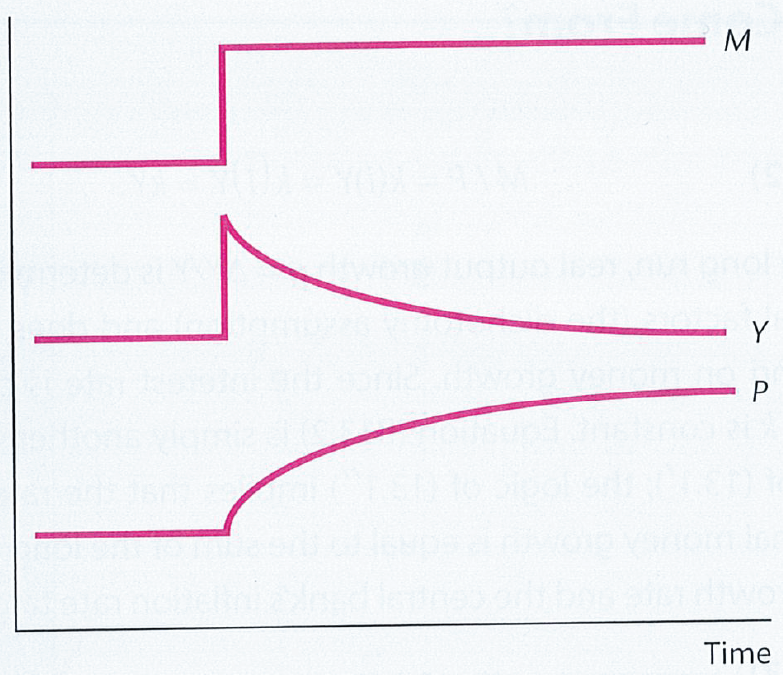
\includegraphics[trim=0 0 0 0,clip,width=0.5\textwidth]{FIGURES/8_ShortLongRun}
%	}      
%	%\subfigure{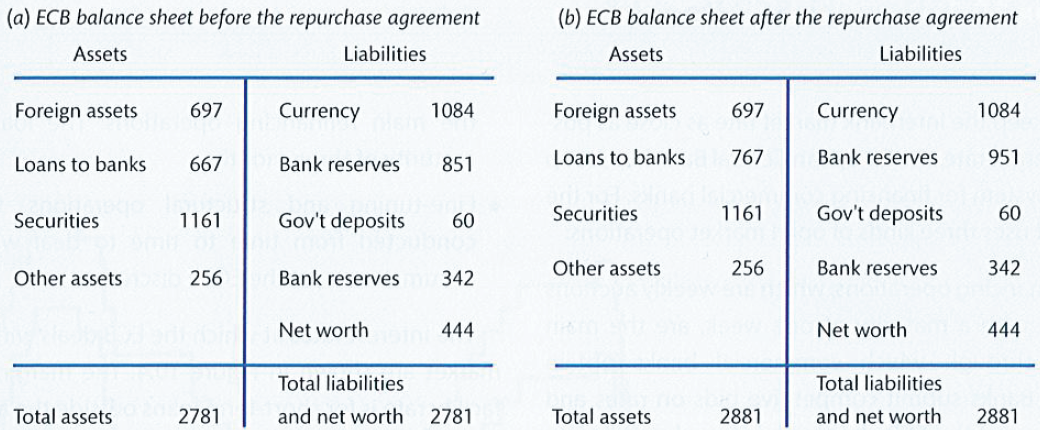
\includegraphics[trim=0 00 0 00,clip,width=0.6\textwidth]{FIGURES/5_CB_balance_sheet_OMO}
%	%} 	
%	%[trim=left bottom right top
%\end{figure}
%%\vspace{-2mm}
%\begin{minipage}{0.5\columnwidth}
%\tiny	
%\textbf{Source.} Burda and Wyplosz (2017), Figure 13.1.\\
%\end{minipage}
%\end{center}
%\end{frame}
%---FRAME------------------------------------------------------------------------------
\begin{frame}{Recap: short vs. long run}

\begin{mytemize}
\item Keynesian short run: supply adjusts to demand
\item Long run: technology, demographics determine output
  \begin{mytemize}
	\item Keynesian demand mechanisms not relevant
  \end{mytemize}
  \begin{center}
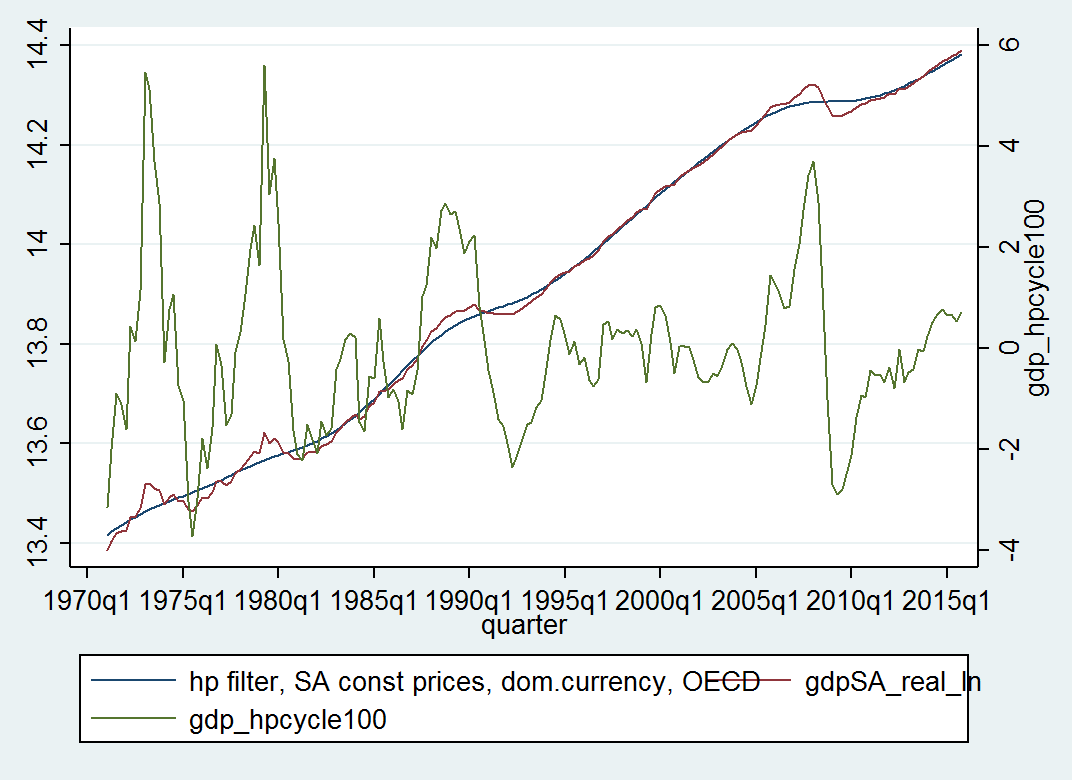
\includegraphics[trim=0 140 0 0,clip,width=0.55\columnwidth]{FIGURES/8_UKoutputDecomp}
\vspace{0.5mm}
%[trim=left bottom right top
\begin{minipage}{1.0\columnwidth}
\tiny	
\textbf{Note.} Decomposition of real GDP in the United Kingdom (in logarithm), 1970Q1 - 2018Q4, using the hp-filter for the trend (blue line) and cycle (green line) decomposition. \textbf{Source.} OECD, author's calculations.
\end{minipage}
  \end{center}

\item[\tb{Next:}] \emph{How do prices and wages move in response to temporary disequilibria on goods and labour markets?}
\end{mytemize}
\end{frame}

\subsection{The Phillips Curve}
%---FRAME------------------------------------------------------------------------------
\begin{frame}
\frametitle{Outline}
\tableofcontents[currentsubsection]
\end{frame}
%---FRAME------------------------------------------------------------------------------
\begin{frame}{Phillips Curve and Okun's law: role for theory}
\begin{mytemize}
\item Keynesian theory: no relation between aggregate output and inflation --- the \emph{missing equation} problem
\item two empirical findings used to fill the theory gap:
  \begin{mynumerate}
	\item A. W. Phillips (1958): negative correlation between wage inflation and unemployment rate
	\item A. Okun (1962): negative correlation between unemployment rate and GDP changes
  \end{mynumerate}
\item[\rarr] inflation-output relationship
\end{mytemize}
\end{frame}
%---FRAME------------------------------------------------------------------------------
\begin{frame}{The Phillips Curve}
\begin{center}
%{\small
%Figure. 
%}
PC in theory \hspace{15mm} PC in the data (UK 1921-1973)
%\vspace{-2mm}
\begin{figure}[h!]
	\subfigure{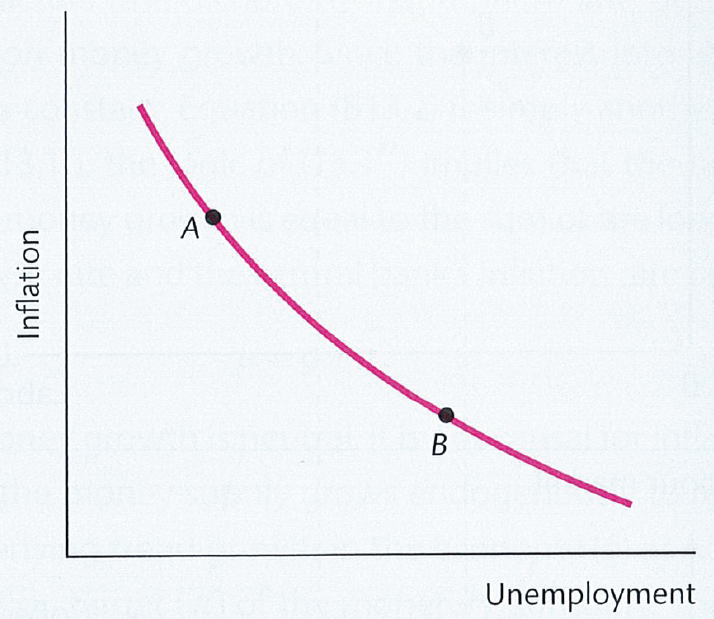
\includegraphics[trim=0 0 0 0,clip,width=0.45\textwidth]{FIGURES/8_PCtheory}
	}      
	\subfigure{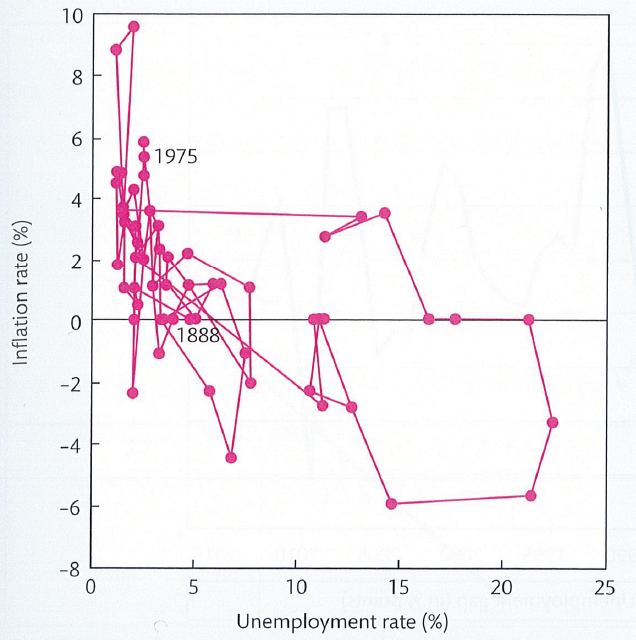
\includegraphics[trim=0 00 0 00,clip,width=0.45\textwidth]{FIGURES/8_PCdataUK}
	} 	
	%[trim=left bottom right top
\end{figure}
%\vspace{-2mm}
\begin{minipage}{1.0\columnwidth}
\tiny	
\textbf{Source.} Burda and Wyplosz (2017), Figure 13.3, Figure 13.4.\\
\end{minipage}
\end{center}

\end{frame}
%---FRAME------------------------------------------------------------------------------
\begin{frame}{The Phillips Curve: policy trade-off}


\begin{mytemize}
\item Phillips curve as an intuitive and practical idea for policy-makers: cannot achieve all good macro indicators at once:
  \begin{mytemize}
\item Either lower inflation and higher unemployemt, ...
\item ... or higher inflation, but lower unemployment.
  \end{mytemize}
\item Slope of Phillips curve referred to as \tb{sacrifice ratio}
\end{mytemize}

\medskip

\medskip

\emph{"I would rather prefer 5\% inflation, then 5\% unemployment (...)"}
\flushright{Helmut Schmidt, 1978}

\end{frame}
%---FRAME------------------------------------------------------------------------------
\begin{frame}{Okun's Law}

\begin{itemize}
\small
\item \emph{Missing element:} Aggregate relationship between output and inflation
\end{itemize}
\begin{align*}
\text{\alert{inflation}} \underset{(1)PC}{\quad \leftarrow \rightarrow \quad} \text{unemployment} \underset{(2)OL}{\quad \leftarrow \rightarrow \quad} \text{\alert{output}}
\end{align*}

\begin{mynumerate}
\small
\item (1)\tb{Phillips curve} (PC) not sufficient
\item (2)\tb{Okun's Law} (OL), Arthur Okun (1928-1980):
\begin{itemize}
\small
\item negative relationship between output and unemployment.
\end{itemize}
\end{mynumerate}


\end{frame}
%---FRAME------------------------------------------------------------------------------
\begin{frame}{Okun's Law: Data}

\begin{itemize}
\small
\item \tb{output gap} and \tb{unemployment gap} are negatively correlated, $corr(Y_{gap},U_{gap})<0$, 
$Y_{gap} \equiv (Y-\bar{Y})/\bar{Y}$ and $U_{gap} \equiv U-\bar{U}$
\item equilibrium level of unemployment, $\bar{U}$
\item potential level of output, $\bar{Y}$
\item Modelling:
\begin{align*}
U_{gap} = -h Y_{gap}
\end{align*}
\end{itemize}

\begin{center}
{\small
Figure. The output gap and unemployment in Germany, 1970-2016
}
%\vspace{-2mm}
\begin{figure}[h!]
%	\subfigure{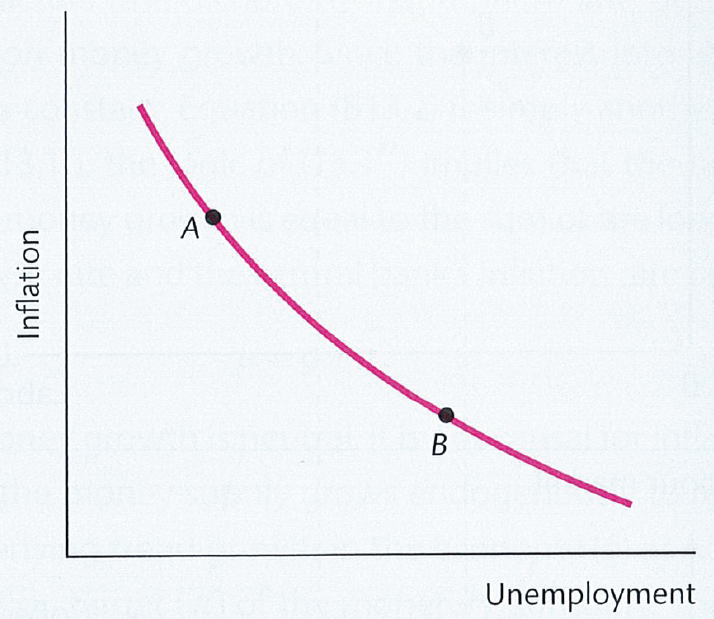
\includegraphics[trim=0 0 0 0,clip,width=0.45\textwidth]{FIGURES/8_PCtheory}
%	}      
	\subfigure{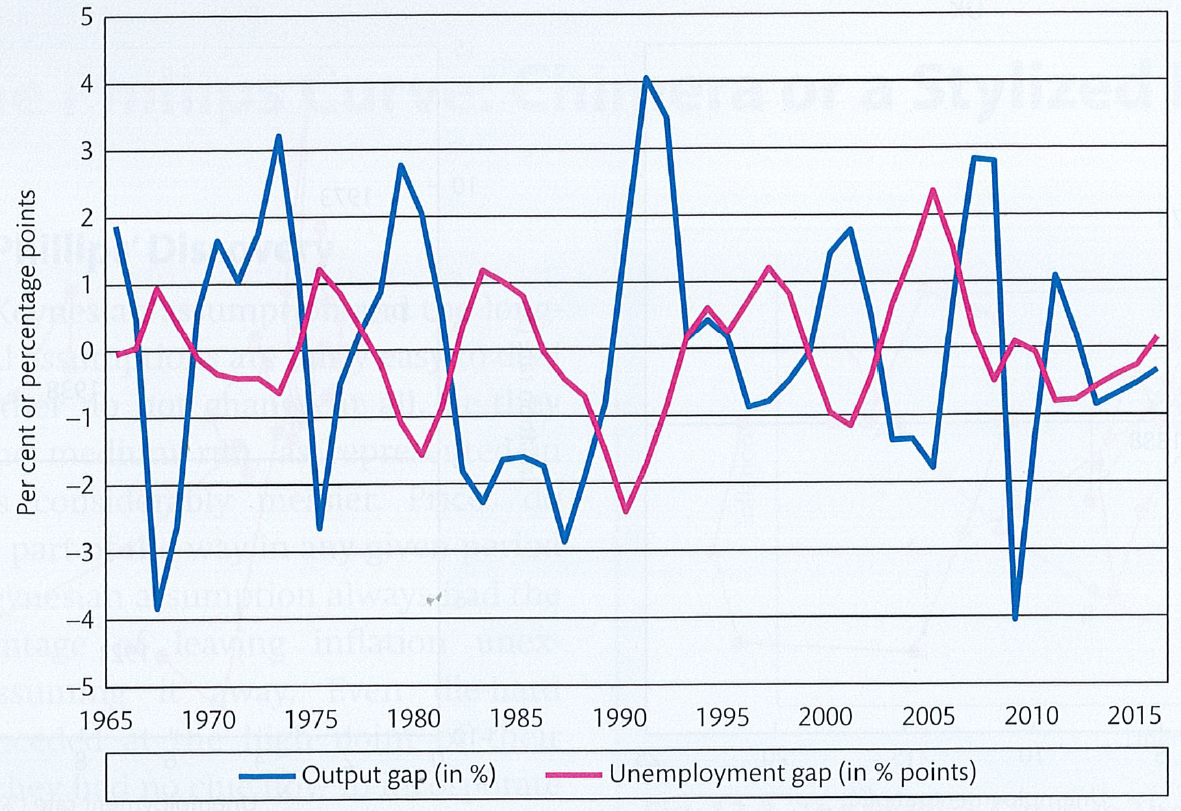
\includegraphics[trim=0 00 0 00,clip,width=0.5\textwidth]{FIGURES/8_OkunsLawDE}
	} 	
	%[trim=left bottom right top
\end{figure}
%\vspace{-2mm}
\begin{minipage}{0.5\columnwidth}
\tiny	
\textbf{Source.} Burda and Wyplosz (2017), Figure 13.5.\\
\end{minipage}
\end{center}

\end{frame}
%---FRAME------------------------------------------------------------------------------
%\begin{frame}{Okun's Law: calibrating h}
%
%\begin{itemize}
%\small
%\item What is the value of $h$ in the data?
%\item US: $\approx -1/3$, Germany: $\approx -1/15$
%\end{itemize}
%
%\begin{center}
%%{\small
%%Figure. The output gap and unemployment in Germany, 1970-2016
%%}
%%\vspace{-2mm}
%\begin{figure}[h!]
%%	\subfigure{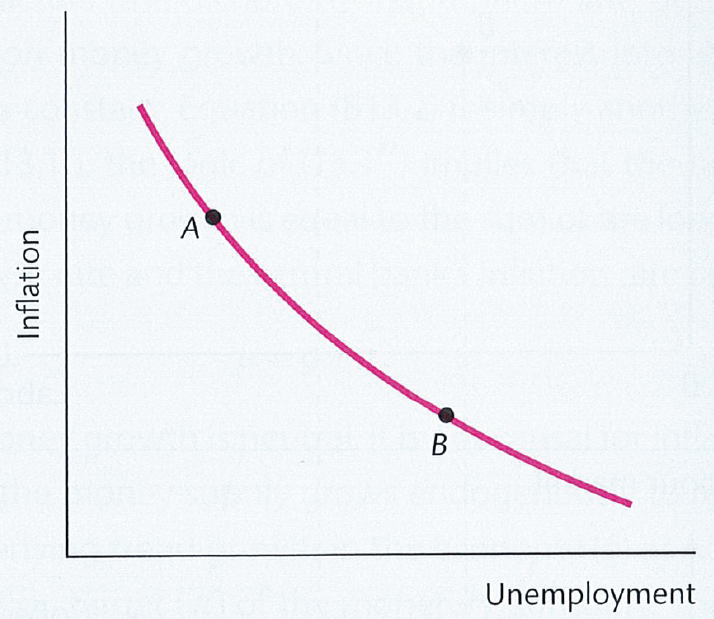
\includegraphics[trim=0 0 0 0,clip,width=0.45\textwidth]{FIGURES/8_PCtheory}
%%	}      
%	\subfigure{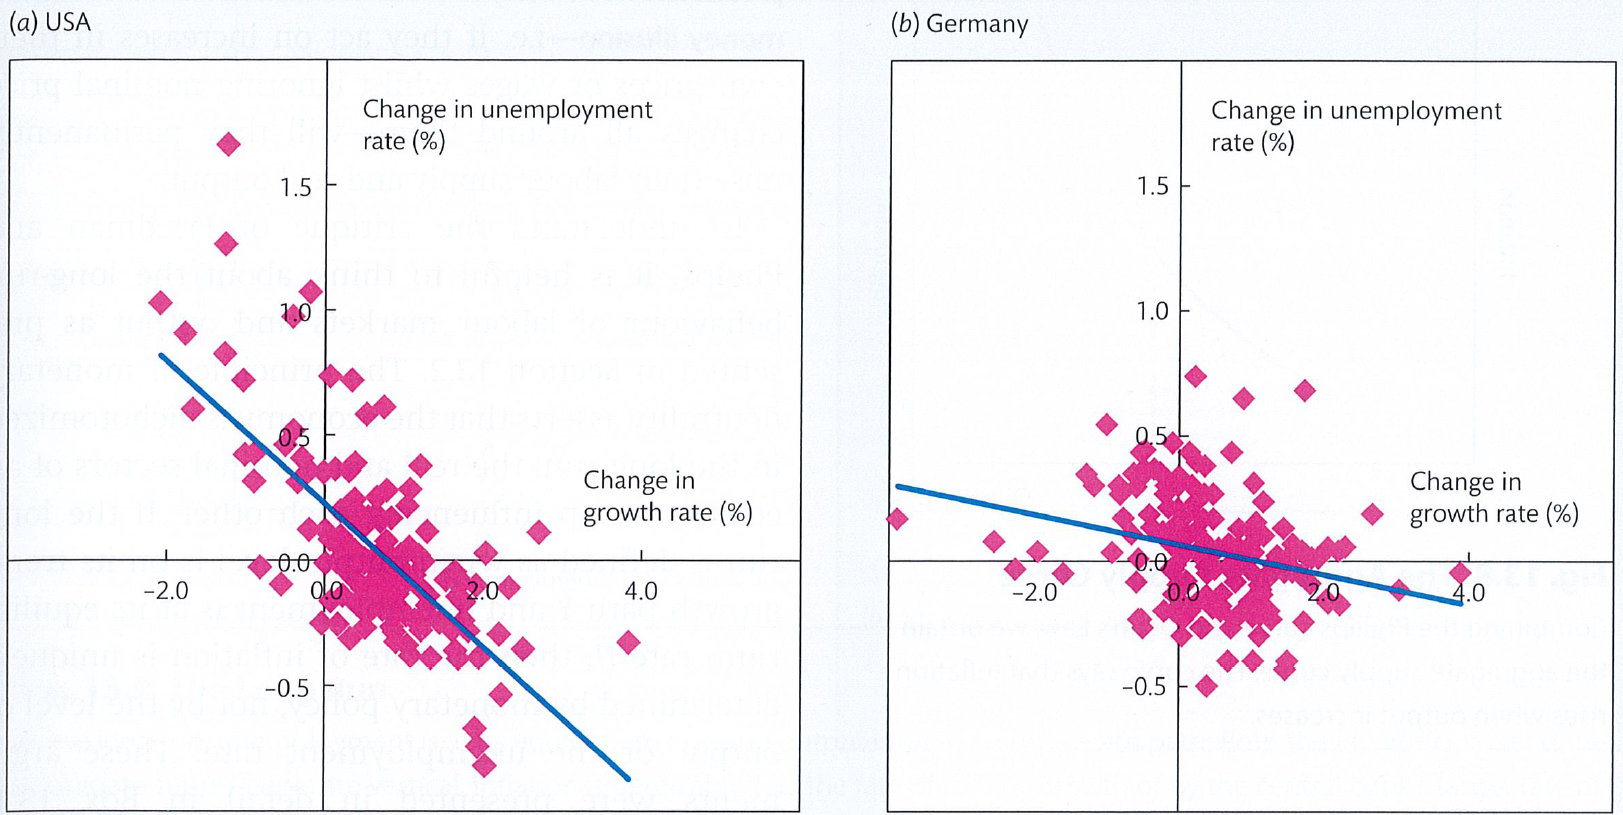
\includegraphics[trim=0 00 0 00,clip,width=0.99\textwidth]{FIGURES/8_OkunsLawCalibrating_h}
%	} 	
%	%[trim=left bottom right top
%\end{figure}
%%\vspace{-2mm}
%\begin{minipage}{0.99\columnwidth}
%\tiny
%\textbf{Note.} Quarterly data, 1971Q1 - 2010Q4, for the USA and Germany. 	
%\textbf{Source.} Burda and Wyplosz (2017), Figure 13.7.\\
%\end{minipage}
%\end{center}
%
%\end{frame}
%---FRAME------------------------------------------------------------------------------
%\begin{frame}{Okun's Law: A Supply Curve Interpretation}
%
%\begin{itemize}
%\small
%\item Combining Phillips curve and Okun's Law: $corr(\pi,(Y-\bar{Y})/\bar{Y})>0$
%\item $\rightarrow$ the \tb{aggregate supply curve}
%\begin{itemize}
%\footnotesize
%\item Under which conditions do firms supply more output and labour?
%\item Analogy to micro supply curve misleading: it is the aggregate level of output on the x-axis, and the rate of change of an index of all prices (inflation) on the y-axis (versus production and price of a single good in micro)
%\end{itemize}
%\end{itemize}
%
%\begin{center}
%%{\small
%%Figure. The output gap and unemployment in Germany, 1970-2016
%%}
%%\vspace{-2mm}
%\begin{figure}[h!]
%%	\subfigure{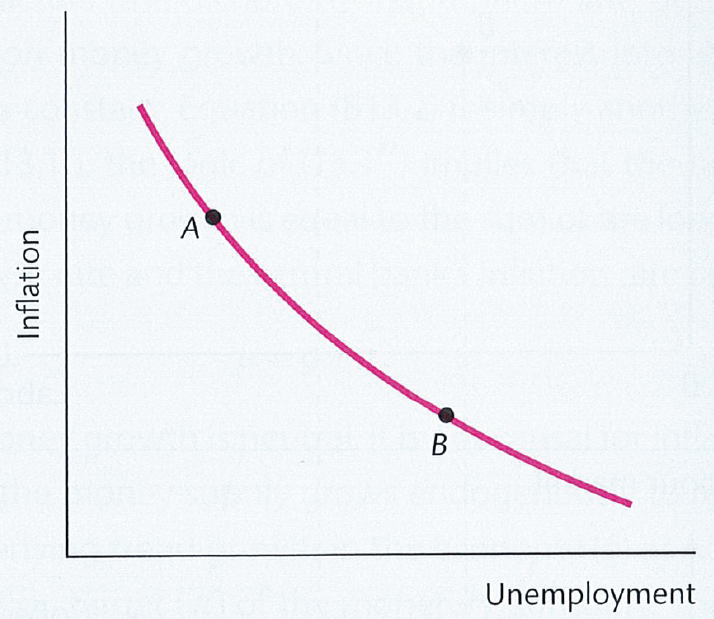
\includegraphics[trim=0 0 0 0,clip,width=0.45\textwidth]{FIGURES/8_PCtheory}
%%	}      
%	\subfigure{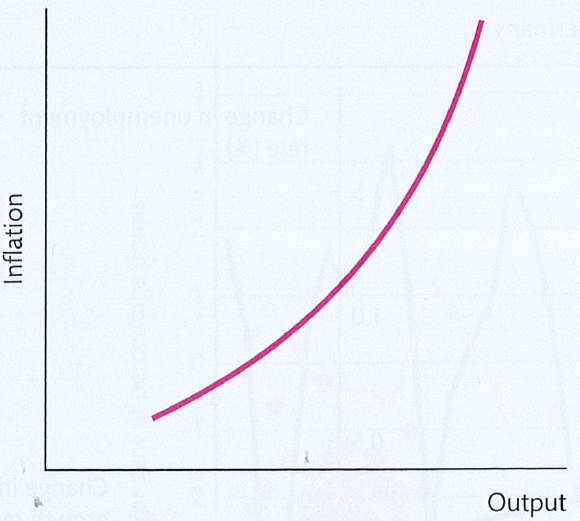
\includegraphics[trim=0 00 0 00,clip,width=0.5\textwidth]{FIGURES/8_AggregateSupplyCurve}
%	} 	
%	%[trim=left bottom right top
%\end{figure}
%%\vspace{-2mm}
%\begin{minipage}{0.50\columnwidth}
%\tiny	
%\textbf{Source.} Burda and Wyplosz (2017), Figure 13.8.\\
%\end{minipage}
%\end{center}
%
%\end{frame}
%---FRAME------------------------------------------------------------------------------
%\begin{frame}{Aggregate Supply}
%
%\begin{align*}
%Y&=A N^{\alpha} \textnormal{ with }0<\alpha<1 \textnormal{ and } A>0 \\
%\bar{Y}&=A\bar{N}^{\alpha}
%\end{align*}
%with $\bar{N}$ is the labor force. Wages depend on price level and the ratio of employment to labor force
%\begin{align*}
%W= \omega P^{\theta}P^{1-\theta}_{-1} \left(\frac{N}{\bar{N}}\right)^{\gamma} \textnormal{ with } 0\leq\theta\leq1, \gamma \geq 0
%\end{align*}
%
%\end{frame}
%---FRAME------------------------------------------------------------------------------
%\begin{frame}{Aggregate Supply}
%
%\begin{itemize}
%\item no full wage indexation if $\theta<1$
%\item \emph{nominal wage rigidity}
%\item $P\uparrow$, $W/P\downarrow$
%\item $\gamma$: bargaining power of labor force $\uparrow$ if $N/\bar{N}\uparrow$
%\end{itemize}
%
%FOC of firms:
%\begin{align*}
%\alpha A N^{\alpha-1} = \frac{W}{P}
%\end{align*}
%
%Thus
%\begin{align*}
%\alpha A N^{\alpha-1}=\omega \left( \frac{P_{-1}}{P}\right)^{1-\theta} \left(\frac{N}{\bar{N}}\right)^{\gamma}
%\end{align*}
%
%\end{frame}
%---FRAME------------------------------------------------------------------------------
%\begin{frame}{Aggregate Supply}
%
%\begin{itemize}
%\item relationship between employment (output) and price level
%\item \tb{Long-run:} $P=P_{-1}$, thus $N=\bar{N}$, $Y=\bar{Y}$ and $W/P=\omega$. Supply curve is \emph{vertical}.
%\item \tb{Short-run:} $P_{-1}$ given
%\begin{align*}
%&Y=HP^{\sigma}, \textnormal{ with } \sigma = \frac{\alpha
%(1-\theta}{1+\gamma-\alpha}>0 \\
%&\textnormal{with a const.} H
%\end{align*}
%\item production pos. depends on prices, since it \emph{reduces the real wage}. $\rightarrow$ upward sloping supply curve!
%\item Price elasticity of supply (slope) depends neg. of degree of wage indexation $\theta$ and responsiveness of the employment level $\gamma$.
%\end{itemize}
%
%\end{frame}
%---FRAME------------------------------------------------------------------------------
%\begin{frame}{Criticism on the Phillips curve}
%\tm{Theoretic foundations}
%\begin{itemize}
%\small
%\item Edmund Phelps and Milton Friedman: Phillips curve only a \tb{temporary phenomenon}
%\item Only under permanent \tb{money illusion}
%\item In the long run, PC and aggregate supply curve must be \emph{vertical}
%\end{itemize}
%\end{frame}
%---FRAME------------------------------------------------------------------------------
%\begin{frame}{Criticism on the Phillips curve: evidence post 1970}
%
%\begin{itemize}
%\small
%\item \tb{stagflation} in many countries, i.e. inflation and absence of output growth
%\item Phillips curve seemed to disappear during \emph{'oil shocks'} (1973/74, 1979/80)
%\item Policy: more emphasis on monetary targeting
%\item Next: Understanding why the Phillips curve 'appears' and 'disappears' \\
%$\rightarrow$ price setting, productivity and the labour share, supply shocks
%\end{itemize}
%%\vspace{-2mm}
%\begin{center}
%{\tiny
%Figure. United Kingdom, 1970-2015
%}
%\vspace{-3mm}
%\begin{figure}[h!]
%%	\subfigure{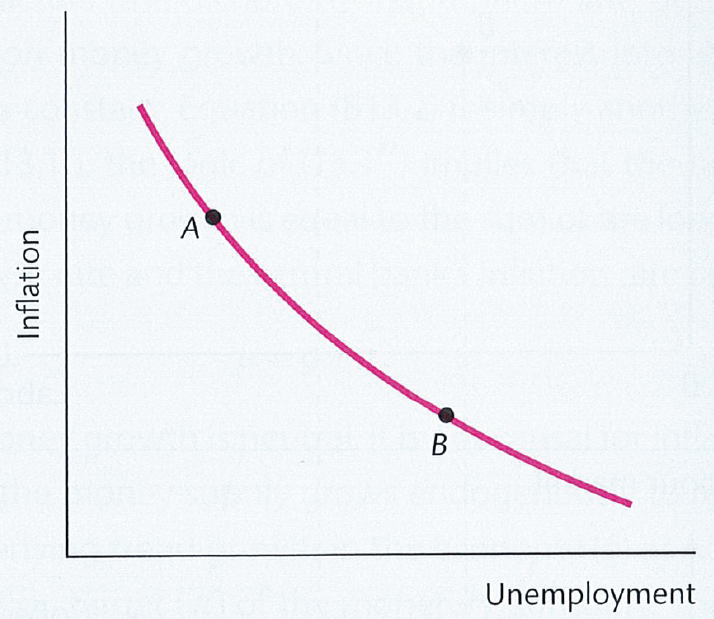
\includegraphics[trim=0 0 0 0,clip,width=0.45\textwidth]{FIGURES/8_PCtheory}
%%	}      
%	\subfigure{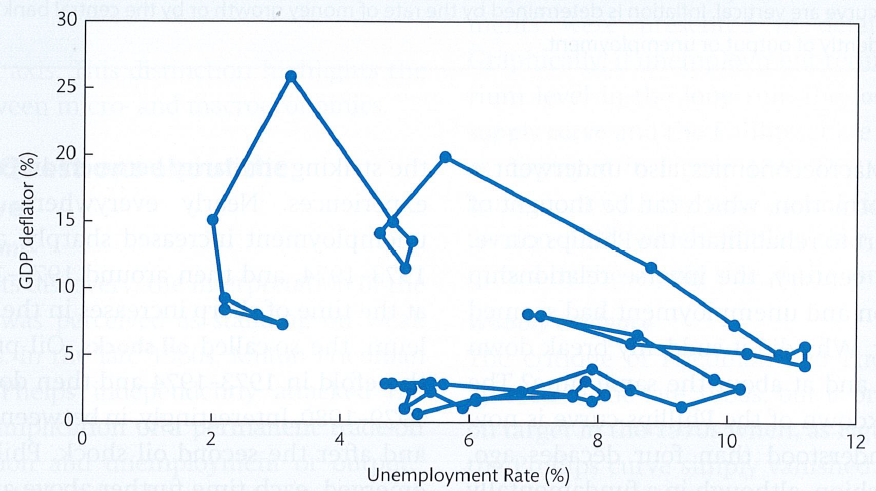
\includegraphics[trim=0 00 0 00,clip,width=0.65\textwidth]{FIGURES/8_PCdataUKpost70}
%	} 	
%	%[trim=left bottom right top
%\end{figure}
%%\vspace{-2mm}
%\begin{minipage}{0.50\columnwidth}
%\tiny	
%\textbf{Source.} Burda and Wyplosz (2017), Figure 13.10.\\
%\end{minipage}
%\end{center}
%
%\end{frame}
%---FRAME------------------------------------------------------------------------------
\subsection{Theoretical Phillips Curve --- markups}
%---FRAME------------------------------------------------------------------------------
\begin{frame}
\frametitle{Outline}
\tableofcontents[currentsubsection]
\end{frame}
\begin{frame}{Prices and Costs}
  How are goods' prices (inflation) connected to wages and to output? Consider profit-maximizing firms:

\begin{mytemize}
\item Firms have some \tb{monopoly power} \rarr set prices
\item Cannot set prices too high because demand is \tb{price-elastic}
\end{mytemize}

\vfill

\tb{Mark-up pricing:}
\begin{itemize}
\small
\item Prices cannot be below \tb{marginal costs}
\item Monopoly power \rarr price = marginal costs + \tb{mark-up}
\item Size of mark-up depends on \tb{demand elasticity}
\item Competitive markets: high elasticity, mark-up $\rightarrow 0$ 
\end{itemize}

\end{frame}
%---FRAME------------------------------------------------------------------------------
\begin{frame}{Marginal cost vs. average cost, share of labor cost}
  If $TC(Y)$ are total costs, \tb{marginal costs} are $\frac{d TC(Y)}{Y}$. \\
  %If labor is the only production factor and production function linear, $TC$ has form $$TC(Y) = c \times Y$$ 
  %where $c > 0$ a positive constant. 
  \tb{Marginal costs} can be approximated by \tr{average costs} or \tr{unit costs} $\frac{TC(Y)}{Y}$:

\begin{align*}
  \text{unit costs} = \frac{TC(Y)}{Y} =
  \underbrace{\frac{W \cdot L}{Y}}_{\text{unit labour costs}} + \underbrace{\frac{\text{total non-labor costs}}{Y}}_{\text{unit non-labor costs}}
\end{align*}
Share of labor costs is firms output --- $S^L$ --- is ratio of labor costs to \textit{value} of output: 
\begin{align*}
  S^L = \frac{W \cdot L}{P \cdot Y}
\end{align*}
Share of labour costs ranges from 50\% to 70\% in firms' output in developed countries and is stable over time --- one of Kaldor's stylized facts.
%
%\begin{center}
%%{\small
%%Figure. The output gap and unemployment in Germany, 1970-2016
%%}
%%\vspace{-2mm}
%\begin{figure}[h!]
%%	\subfigure{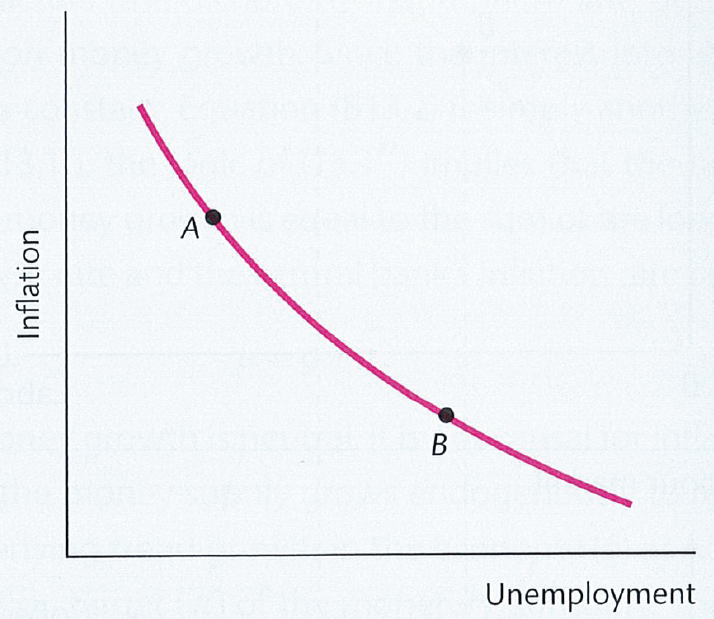
\includegraphics[trim=0 0 0 0,clip,width=0.45\textwidth]{FIGURES/8_PCtheory}
%%	}      
%	\subfigure{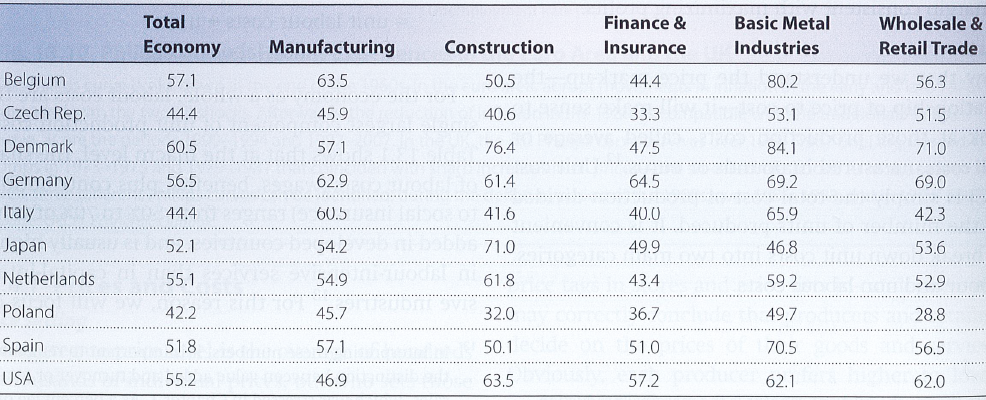
\includegraphics[trim=0 00 0 00,clip,width=0.7\textwidth]{FIGURES/8_LabourShare}
%	} 	
%	%[trim=left bottom right top
%\end{figure}
%%\vspace{-2mm}
%\begin{minipage}{0.50\columnwidth}
%\tiny	
%\textbf{Note.} Wage share of value added by country and selected industries, 2014. \textbf{Source.} Burda and Wyplosz (2017), Table 13.1.\\
%\end{minipage}
%\end{center}
\end{frame}
%---FRAME------------------------------------------------------------------------------
\begin{frame}{Building theoretical Phillips curve: battle of markups}
\tb{Prices as mark-up on labour costs}\\
Firms with market power aim to set price as a markup over unit labor cost (or setting labor cost share):
\begin{align*}
P = (1+\theta) \frac{WL}{Y},
\end{align*}
where $\theta>0$ the markup.\\
\vfill
\tb{Wages as a mark-up on prices}\\
Workers (unions) bargain with firms for higher wages. \tr{Sticky wages}: negotiated wage fixed for some periods \rarr firms exposed to change of $\frac{W}{P}$ in the future under a fixed $W$ \rarr $P^e$ used in wage setting.  Bargaining determines firms' labor cost share under expected future prices $P^e$. In the negotiation, firms have reference price $\bar P$ and workers have reference (minimum) wage $\bar W$.
\begin{align*}
\frac{WL}{Y} = (1+\gamma)\bar{S}_L P^e,
\end{align*}
where $\bar{S}_L$ is reference labor cost share $\bar{S^L} = \frac{\bar W L}{\bar P Y}$ and $\gamma$ is the markup.
\end{frame}
\begin{frame}{Microfoundations: price setting}
  \vspace{-3cm}
  \small
  \begin{columns}
	\column{0.4\linewidth}
  \vspace{-0.5cm} $\underset{P}{\max} \ P \cdot Y - W \cdot L$, with \\
	\column{0.6\linewidth}
  $Y = Y^d(P)$ consumers' goods demand, \\ $L = L^d(Y)$ firm's  labor demand.
  \end{columns}
  \vfill
\end{frame}

\begin{frame}{Microfoundations: wage setting}
  \vspace{-3cm}
  \small \hspace{-0.5cm} $\underset{W}{\max} \ (W - \bar W)^\beta (\bar P \cdot Y - W \cdot L)^{1-\beta}$, where $\beta$ is workers' negotiation power.
  \vfill
\end{frame}

%---FRAME------------------------------------------------------------------------------
\begin{frame}{Building theoretical Phillips curve: battle of markups}

\begin{mytemize}
\item Prices depend on wage, wage depends on \tr{expected} prices
\item[\rarr] combining wage setting and price setting equations, dependence of current wages on future wage obtained
\begin{align*}
P = (1+\theta)(1+\gamma)\bar{S}_L P^e
\end{align*}
\item anchor: expected price level $P^e$
\end{mytemize}
\end{frame}
%---FRAME------------------------------------------------------------------------------
\begin{frame}{From markups to output and unemployment}
\begin{align*}
P = (1+\theta)(1+\gamma)\bar{S}_L P^e
\end{align*}
The product $(1+\theta)(1+\gamma)$ most likely \emph{procyclical}.
\begin{mytemize}
\item Price markup $\theta$: when GDP rises, competition increases ($\theta \downarrow$), but demand elasticity decreases ($\theta \uparrow$)
  \begin{mytemize}
  \item[\rarr] total effect mixed
  \end{mytemize}
\item Wage markup $\gamma$: when GDP rises, higher workers' bargaining power ($\beta$), firms hire and incentivise over-time work ($\gamma \uparrow$)
  \begin{mytemize}
  \item[\rarr] $\gamma$ procyclical
  \end{mytemize}
\end{mytemize}
\end{frame}
%---FRAME------------------------------------------------------------------------------
\begin{frame}{From price to inflation: deriving AS and Phillips curve}
  Taking logs and total differential of the equation:
\begin{align*}
P &= (1+\theta)(1+\gamma)\bar{S}_L P^e \\
\ln P &= \theta+\gamma+\ln \bar{S}_L + \ln P^e \ (\text{as} \ \ln(1+x)\underset{x \to 0}{\to} x)\\
\text{total differential:} \frac{d P}{P} &= d \theta + d \gamma + \underbrace{\frac{d \bar S^L}{\bar S^L}}_{=0} + \frac{d P^e}{P^e} \\
\pi &= d \theta + d \gamma + \pi^e
\end{align*}
$\theta + \gamma$ \tb{procyclical} $\rightarrow d \theta + d \gamma = a \cdot Y^{gap}$ \rarr 
$$\pi = a \cdot Y_{gap}+ \pi^e$$ 
Finally, using \tb{Okun's law} to replace $Y^{gap}$ with $U^{gap}$:
$$\pi = -b \cdot U_{gap}+ \pi^e$$ 
\end{frame}

\begin{frame}{AS, Phillips Curve --- final form}
  Two elements are added to obtain full \tb{Phillips curve} and \tr{Aggregate Supply} relationships:
\begin{mynumerate}
\item Underlying rate of inflation $\tilde{\pi}$
\begin{mytemize}
\item generalization of expected inflation rate $\pi^e$ in wage setting 
\item wages sticky \rarr not only current expectations, but past expectations influence wage setting
\item explicit rules might exist for adjusting $W$ to $\pi$ \rarr past inflation rates enter $\tilde \pi$
\end{mytemize}
\item Supply shocks $s$
\begin{mytemize}
\item Shocks to non-wage marginal costs
\item Taken into account by firms when setting prices 
\end{mytemize}
\end{mynumerate}
\textbf{Results:}
\begin{align}
  \pi =& -b U_{gap} + \tilde{\pi} + s \tag{Phillips Curve}\\
\pi =& \quad a Y_{gap} + \tilde{\pi} + s \tag{AS}
\end{align}
\end{frame}

\begin{frame}{AS and Phillips curve: symmetry}
\begin{align}
  \pi =& -b U_{gap} + \tilde{\pi} + s \tag{Phillips Curve}\\
\pi =& \quad a Y_{gap} + \tilde{\pi} + s \tag{AS}
\end{align}
  \begin{center}
%{\small
%Figure. The output gap and unemployment in Germany, 1970-2016
%}
%\vspace{-2mm}
\begin{figure}[h!]
%	\subfigure{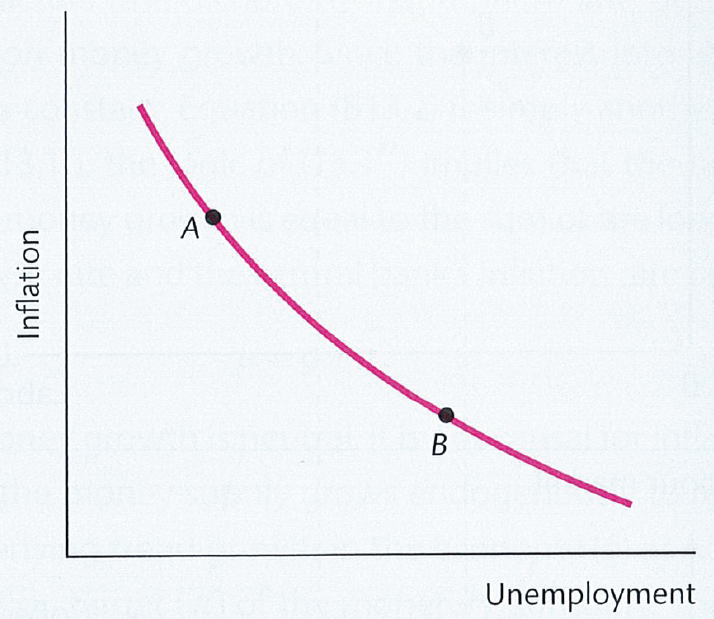
\includegraphics[trim=0 0 0 0,clip,width=0.45\textwidth]{FIGURES/8_PCtheory}
%	}      
	\subfigure{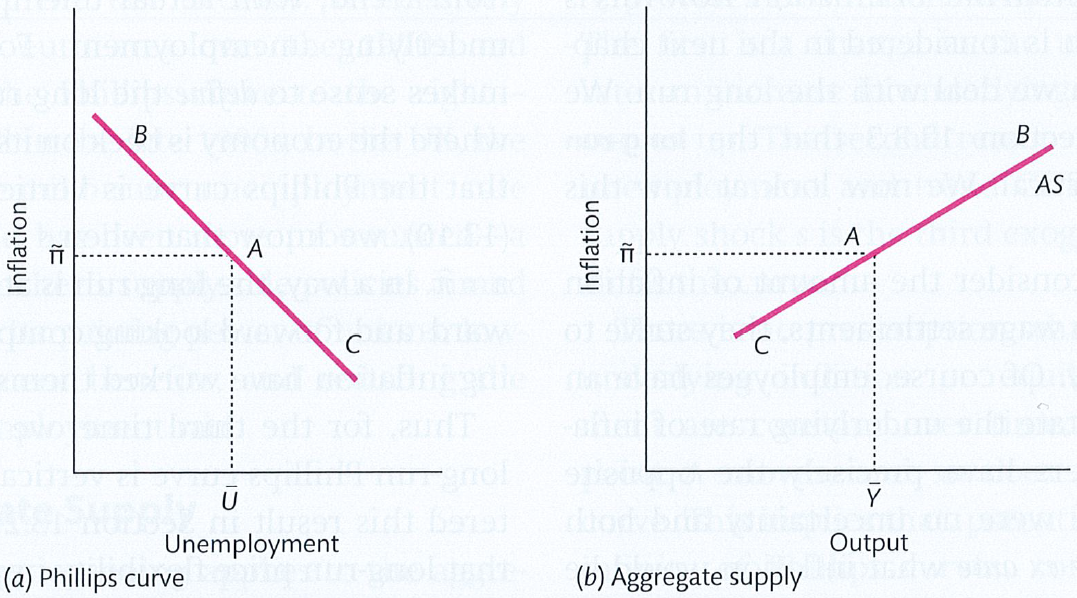
\includegraphics[trim=0 00 0 00,clip,width=0.9\textwidth]{FIGURES/8_NewPC}
	} 	
	%[trim=left bottom right top
\end{figure}
%\vspace{-2mm}
\begin{minipage}{0.90\columnwidth}
\tiny	
\textbf{Note.} The new Phillips curve. \textbf{Source.} Burda and Wyplosz (2017), Figure 13.12.\\
\end{minipage}
\end{center}
\end{frame}
%---FRAME------------------------------------------------------------------------------
\begin{frame}{Non-labour costs and supply shocks}

  Firms have small supply shocks all the time, but which ones are macroeconomic? \\
  \vfill
  \tr{Energy prices}, especially fossil fuels, have a big role:
\begin{itemize}
\item First oil shocks: 1973/74, 1979/81
\item Second sequence of shocks: 1999/2001, 2005/12
\item Favourable oil shocks: 1986 and 2015
\item Current: war \& sanctions \rarr Russian oil shut off: 2022
\end{itemize}

\begin{center}
  \begin{figure}[h]
	\centering
	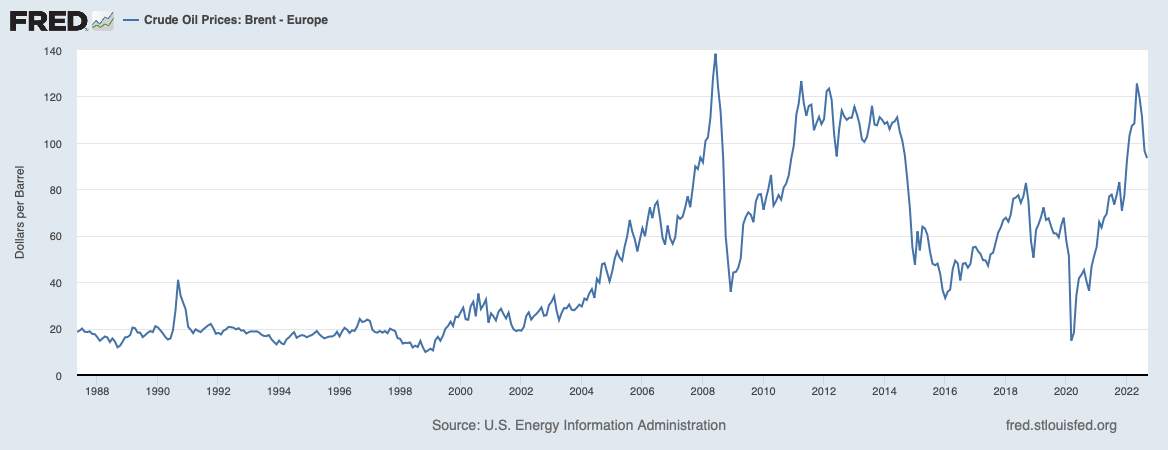
\includegraphics[width = \textwidth]{FIGURES/brent_190922.png}
  \end{figure}
\begin{minipage}{0.5\columnwidth}
\tiny	
Brent Europe crude oil price. \textbf{Source.} St. Louis Fed. \\
\end{minipage}
\end{center}
%\begin{center}
%{\small
%Figure. The output gap and unemployment in Germany, 1970-2016
%}/
%\vspace{-2mm}
\end{frame}
%---FRAME------------------------------------------------------------------------------
\begin{frame}{Underlying inflation, long-run Phillips curve}

\begin{mytemize}
\item \tb{Rational expectations} 
\begin{itemize}
\item Forecast errors occur, but must average to zero over longer horizons
\item Differences in $\pi$ and $\tilde{\pi}$ must be temporary
\item Long-run link equivalence of actual and underlying inflation:\\
if $s=0$ and $U=\bar{U}$, then $\pi=\tilde{\pi}$
\end{itemize}
\item Implies a \tr{vertical Phillips Curve in the long run}
\item The level of \tr{long run inflation}? 
  \begin{mytemize}
  \item[$\rightarrow$] $\bar \pi$, \tr{inflation target of the central bank}.
  \end{mytemize}
\end{mytemize}
\end{frame}
%---FRAME------------------------------------------------------------------------------
\begin{frame}{Long-run Aggregate Supply (LAS)} 

\begin{mytemize}
  \item Recall that \tb{trend output} $\bar Y$ determined by technology, demographics
	\begin{mytemize}
	\item No relation of $\bar Y$ level to $\pi$ \rarr \tr{vertical LAS}
	\end{mytemize}
\item Another way to obtain --- long-run Phillips curve \& Okun's law 
%\item It shifts with changes in exogenous variables ($\tilde{\pi},\bar{Y},s$)
  \end{mytemize}
 \textbf{Implications:}
\begin{mytemize}
\item \tm{Short run}: Actual inflation deviates from underlying inflation $\tilde{\pi}$ in tandem with the business cycle
\item \tm{Long-run}: output returns to its growth path, independent of price level. 
  \begin{mytemize}
  Horizontal movement due to trend output $\bar{Y}$ growing at rate $g$
  \end{mytemize}
\end{mytemize}

\end{frame}
%---FRAME------------------------------------------------------------------------------
\begin{frame}{Shifts in Phillips curve and AS --- unstable relationships}

\begin{mytemize}
\item $\tilde{\pi},\bar{U},\bar{Y},s$ are taken as exogenous and can shift the curves
\item[$\rightarrow$] a set of Phillips curves, not a stable negative relationship
\item A. W. Phillips was \textbf{lucky} to find one stable curve
\item At least to strong reasons for shifts since 1970s:
\begin{mytemize}
\item Supply shocks (oil prices)
\item Shifts in the equilibrium unemployment rate
\end{mytemize}
\end{mytemize}
\begin{center}
{\tiny
Figure. United Kingdom, 1970-2015
}
\vspace{-3mm}
\begin{figure}[h!]
%	\subfigure{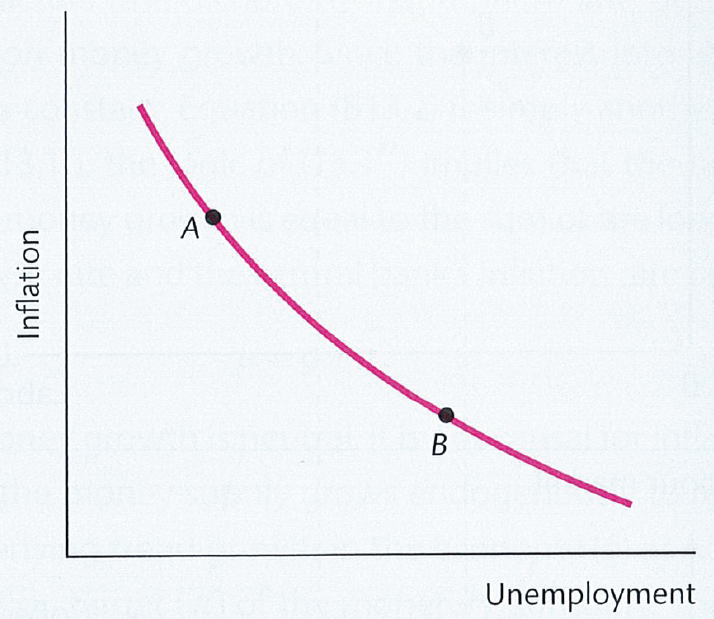
\includegraphics[trim=0 0 0 0,clip,width=0.45\textwidth]{FIGURES/8_PCtheory}
%	}      
	\subfigure{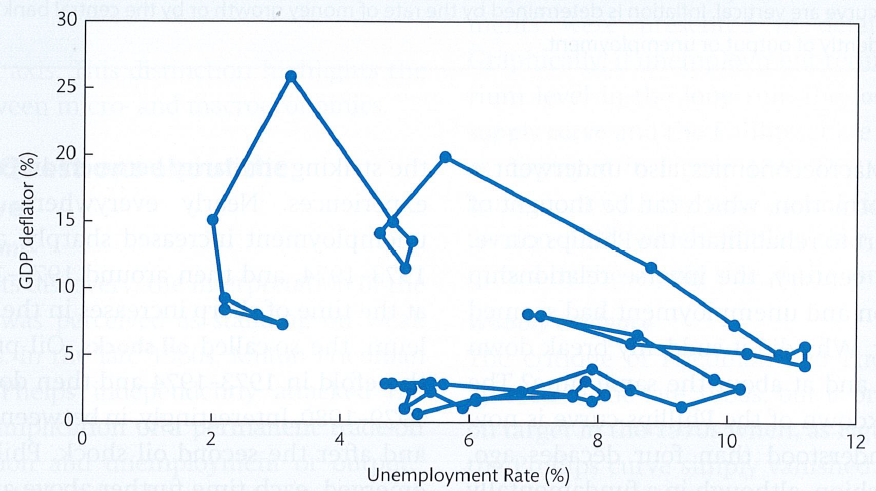
\includegraphics[trim=0 00 0 00,clip,width=0.55\textwidth]{FIGURES/8_PCdataUKpost70}
	} 	
	%[trim=left bottom right top
\end{figure}
%\vspace{-2mm}
\begin{minipage}{0.50\columnwidth}
\tiny	
\textbf{Source.} Burda and Wyplosz (2017), Figure 13.10.\\
\end{minipage}
\end{center}

\end{frame}
%---FRAME------------------------------------------------------------------------------
%\begin{frame}{Changes in equilibrium unemployment over time}
%
%\begin{itemize}
%\small
%\item Upward trend: 1970-2000/10
%\item Downward trend: 2000/10-2015
%\end{itemize}
%\begin{center}
%%{\small
%%Figure. The output gap and unemployment in Germany, 1970-2016
%%}
%%\vspace{-2mm}
%\begin{figure}[h!]
%%	\subfigure{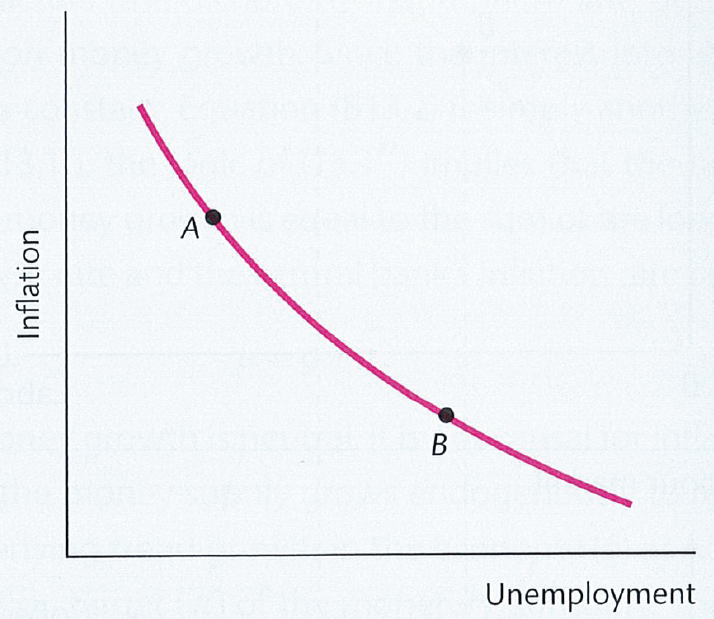
\includegraphics[trim=0 0 0 0,clip,width=0.45\textwidth]{FIGURES/8_PCtheory}
%%	}      
%	\subfigure{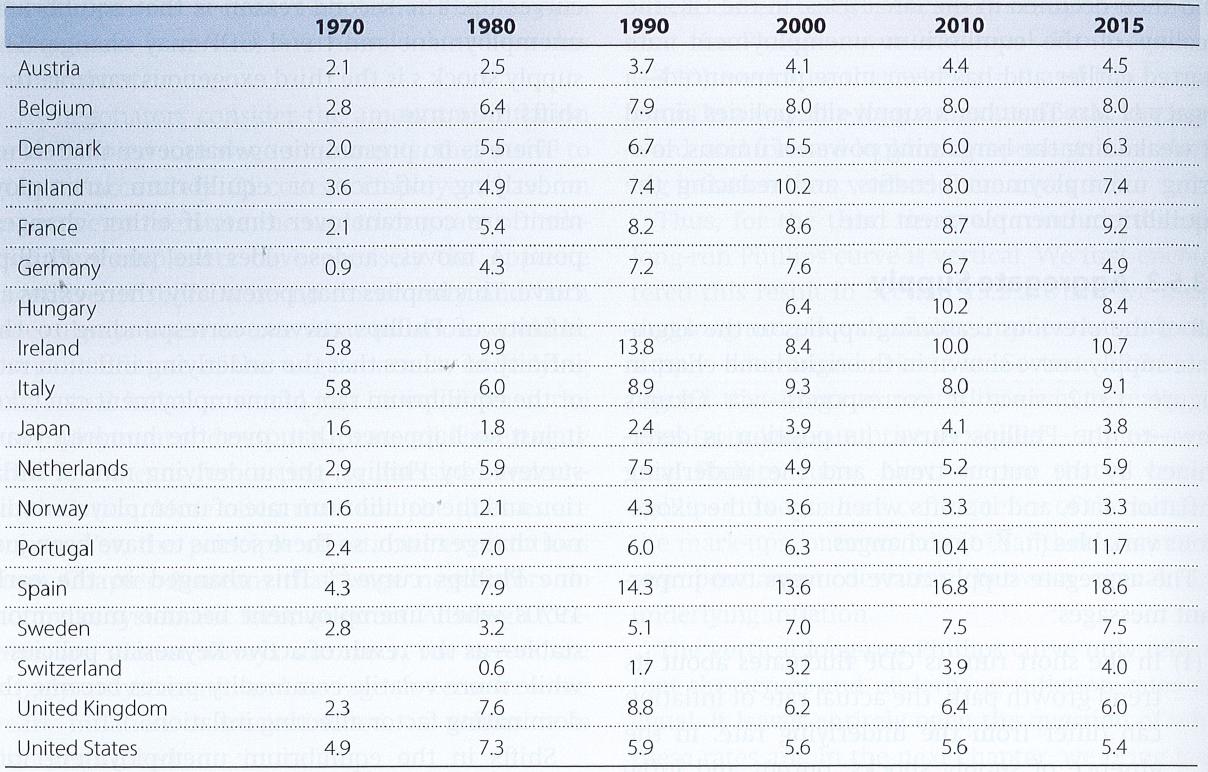
\includegraphics[trim=0 00 0 00,clip,width=0.85\textwidth]{FIGURES/8_TableNAIRU}
%	} 	
%	%[trim=left bottom right top
%\end{figure}
%%\vspace{-2mm}
%\begin{minipage}{0.90\columnwidth}
%\tiny	
%\textbf{Note.} NAIRU = nonaccelerating inflation rate of unemployment (What unemployment rate would keep the Phillips curve unchanged if $\tilde{\pi}=\pi$ and $s=0?$). \textbf{Source.} Burda and Wyplosz (2017), Table 13.2.\\
%\end{minipage}
%\end{center}
%
%\end{frame}
%---FRAME------------------------------------------------------------------------------
\begin{frame}{Phillips curve and AS: summary} 
\begin{mytemize}
\item Instead of a simple $U, \pi$ relationship found originally, theoretical Phillips curve is more flexible:
\begin{mynumerate}
\item Short-run Phillips curve depends on expectations and supply shocks
\item Long-run Phillips curve is vertical --- no inflation-unemployment link
\end{mynumerate}
\item Via \tb{Okun's law}, short-run and long-run \tb{AS} are obtained
\end{mytemize}

\begin{center}
\begin{figure}[h!]
%	\subfigure{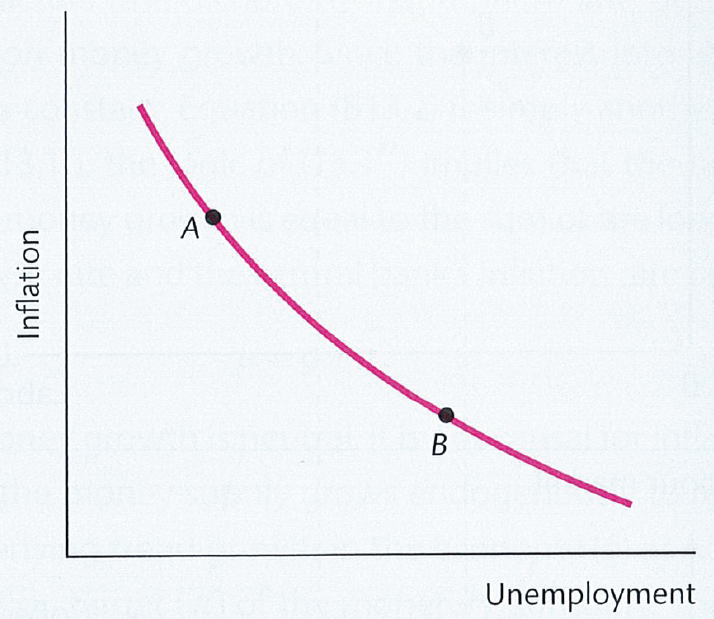
\includegraphics[trim=0 0 0 0,clip,width=0.45\textwidth]{FIGURES/8_PCtheory}
%	}      
	\subfigure{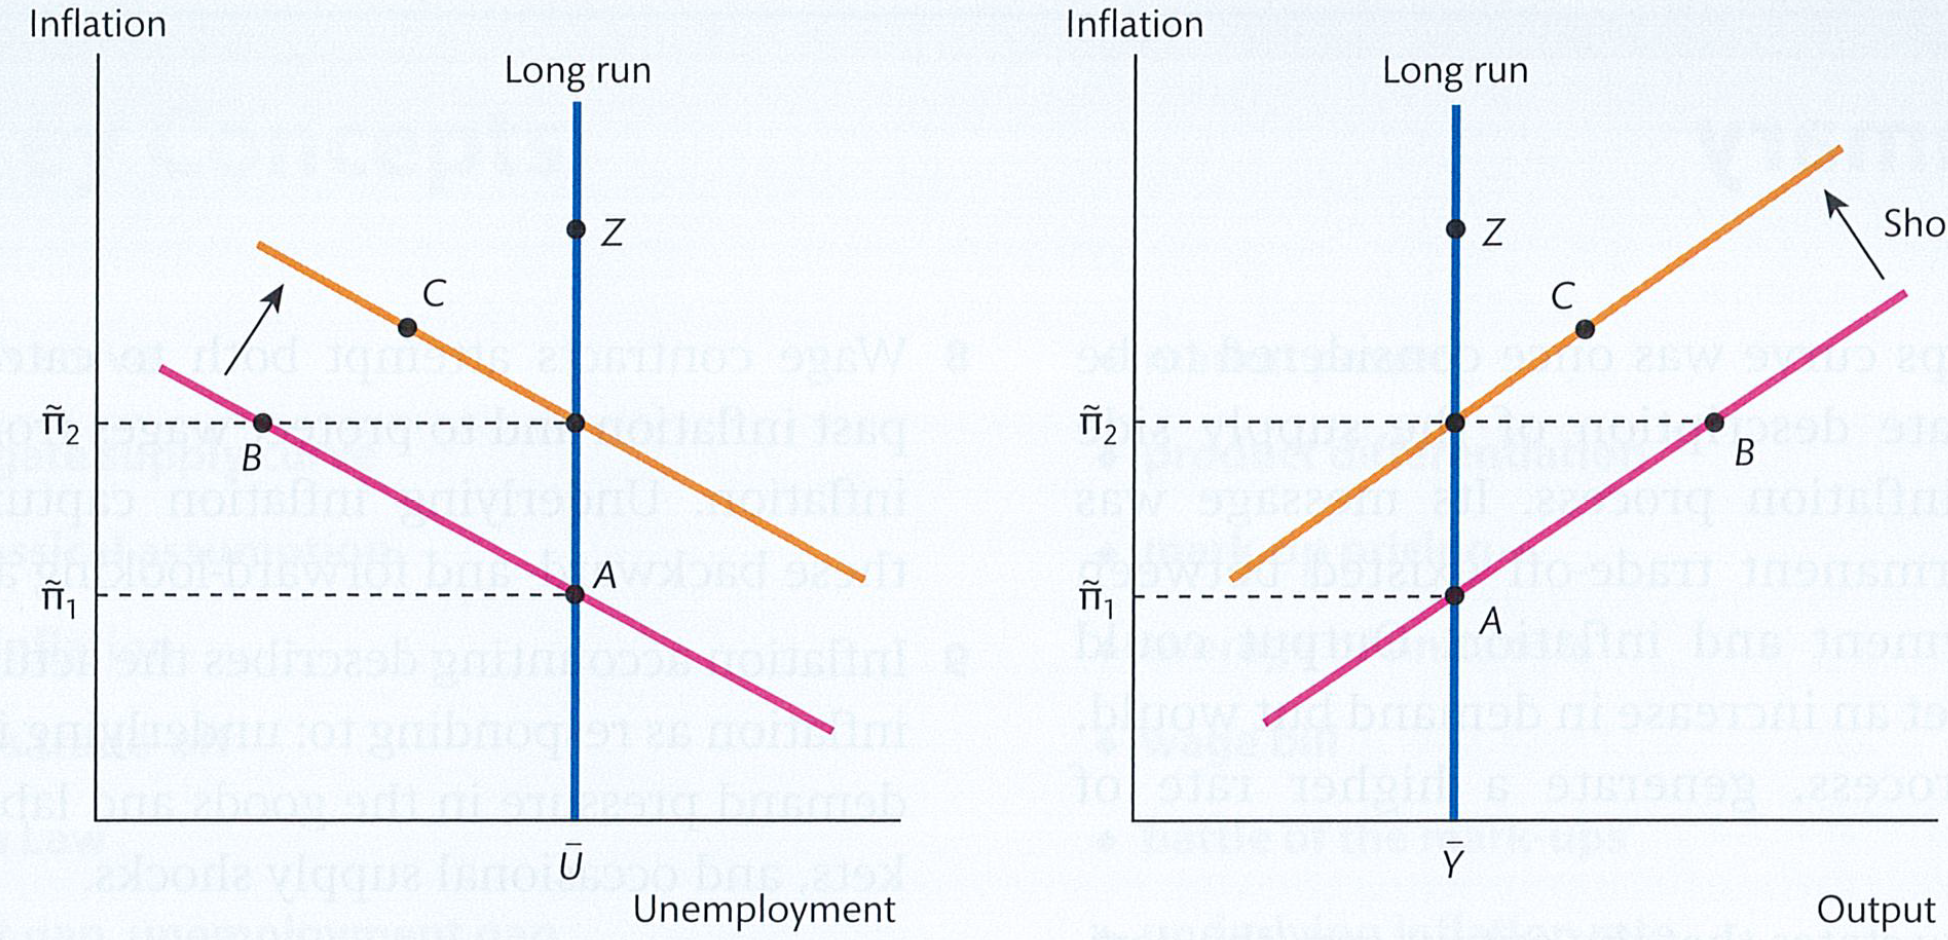
\includegraphics[trim=0 0 0 0,clip,width=0.9\textwidth]{FIGURES/8_TransitionShortLong}
	} 	
	%[trim=left bottom right top
\end{figure}
\vspace{-2mm} \begin{minipage}{0.50\columnwidth}
\tiny	
\textbf{Source.} Burda and Wyplosz (2017), Figure 13.13.\\
\end{minipage}
\end{center}
\end{frame}
%---FRAME------------------------------------------------------------------------------
\section{AS-AD model}
%---FRAME------------------------------------------------------------------------------
%---FRAME------------------------------------------------------------------------------
%\subsection{AS-AD}
%---FRAME------------------------------------------------------------------------------
%\begin{frame}
%\frametitle{Outline}
%\tableofcontents[currentsubsection]
%\end{frame}
%---FRAME------------------------------------------------------------------------------
%\begin{frame}{AS-AD}
%
%
%%\tb{Overview}
%%\begin{itemize}
%%\small
%%\item Monetary policy: exogenous
%%\item Exchange rate: endogenous
%%\end{itemize}
%
%\medskip
%\tb{Steps of our analysis}
%\begin{mytemize}
%\small
%\item \emph{How does aggregate demand work?}
%\begin{itemize}
%\small
%\item Natural rate of interest
%\item AD in the long run
%\item AD in the short run
%\end{itemize}
%\item The complete system
%\begin{itemize}
%\small 
%\item short run
%\item medium run
%\item long run
%\end{itemize}
%\item Policy example: Monetary policy
%\end{mytemize}
%
%
%\end{frame}
%---FRAME------------------------------------------------------------------------------
\begin{frame}{AD-AS model}
  \begin{mytemize}
  \item Medium-term movements of output and inflation shaped by both supply and demand
  \item \tb{AS} is obtained above
  \item \tr{AD} follows immediately from the IS-TR model with full version of TR:
	$$i = \bar i + \textcolor{red}{a(\pi - \bar \pi)} + b\left(\frac{Y- \bar Y}{\bar Y}\right)$$
  \end{mytemize}
\end{frame}


\begin{frame}{Long-run AD: Natural rate of interest}
  \begin{mytemize}
	\item In the long run, central bank assumed to set interest such that $\pi = \bar \pi$ for whatever $Y$ (which is $\bar Y$ anyways) 
	\begin{mytemize}
	\item horizontal \tb{LAD}
	\item will become more relevant in open economy analysis
	\end{mytemize}
  \end{mytemize}
\begin{center}
%{\footnotesize
%Figure. Exchange rate of Danish krona vis-a-vis (a) EUR and (b) USD  \\
%}
%\vspace{-2mm}
\begin{figure}[h!]
%\caption{Figure. Net}
	\subfigure{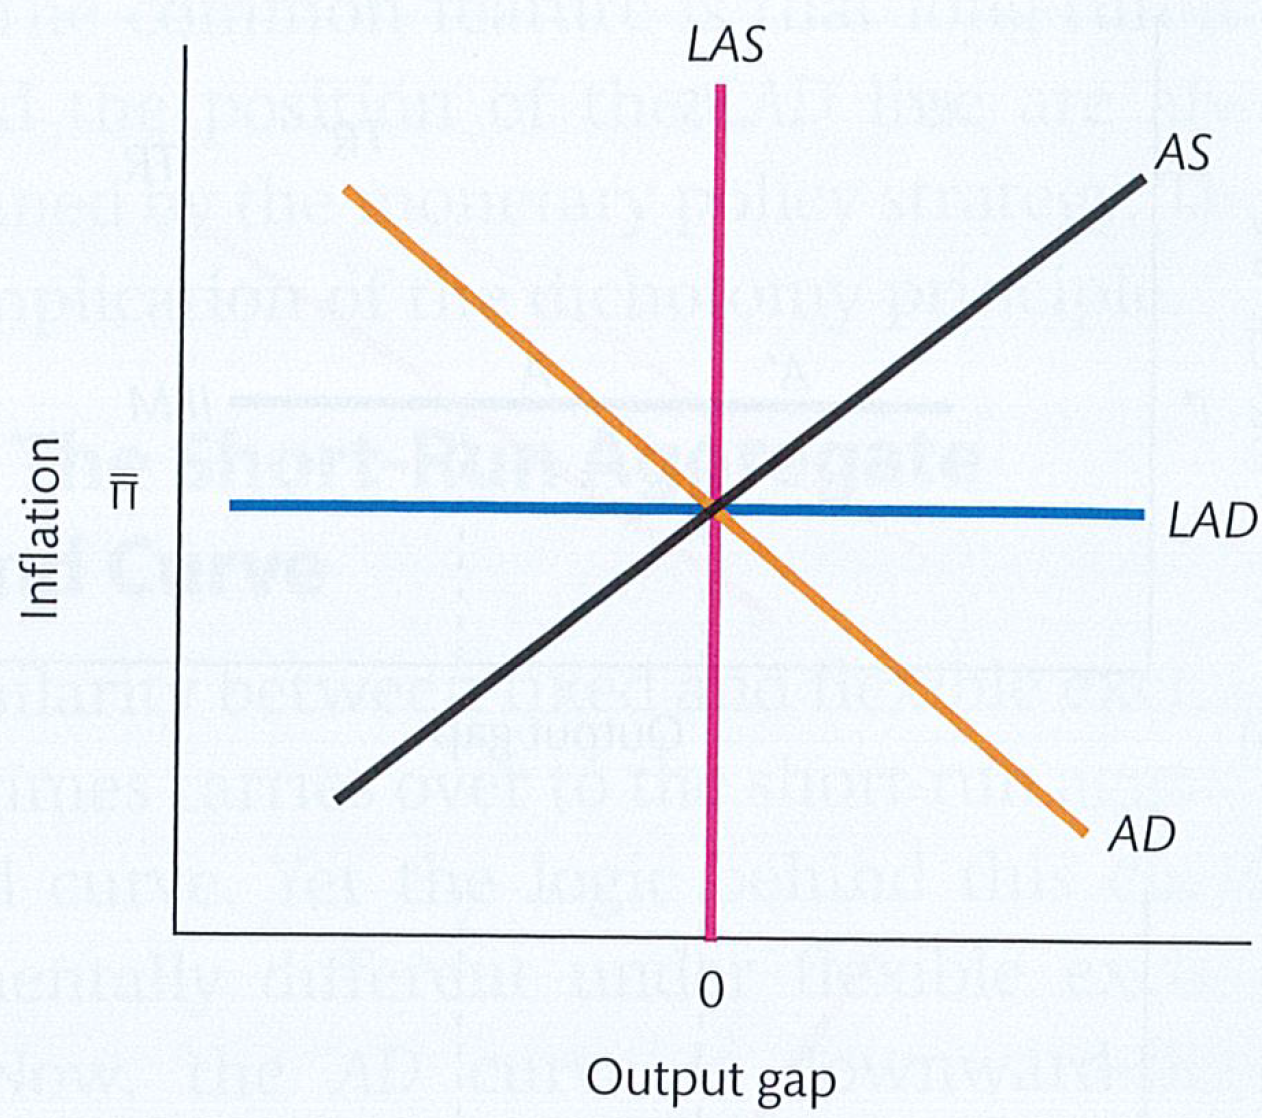
\includegraphics[trim=0 0 0 0,clip,width=0.45\textwidth]{FIGURES/9_ASAD_Flexible}
	}      
	%} 		
%	\label{fig:GPD} 
	%[trim=left bottom right top
\end{figure}
%\vspace{-2mm}
\begin{minipage}{0.5\columnwidth}
\tiny	
%\textbf{Note.} Inflation in Denmark and the euro area (1992-2016).  
\textbf{Source.} Burda \& Wyplosz (2017), Figure 14.12.\\
\end{minipage}
\end{center}
\end{frame}
%---FRAME------------------------------------------------------------------------------
%---FRAME------------------------------------------------------------------------------
\begin{frame}{Short run AD}

\begin{columns}
\column{0.5\linewidth}
Assume an increase in $\pi$:
\begin{itemize}
  \item TR: Central bank raises interest rate 
\item Investment decreases, $IS$ shifts to the left
\item Equilibrium $Y$ lower for higher $\pi$: downward sloping short run \tb{AD}
\end{itemize}
\tb{Shifts in AD}
\begin{itemize}
  \item IS: any shift in desired demand
  \item \emph{TR}: $\bar Y, \bar{\pi}$
%\item \emph{IFM}: $\Delta i^* \neq 0$
\end{itemize}
% COLUMN(2)
\column{0.45\linewidth}
\vspace{7cm}
 AD \& IS-TR:
%\centering
%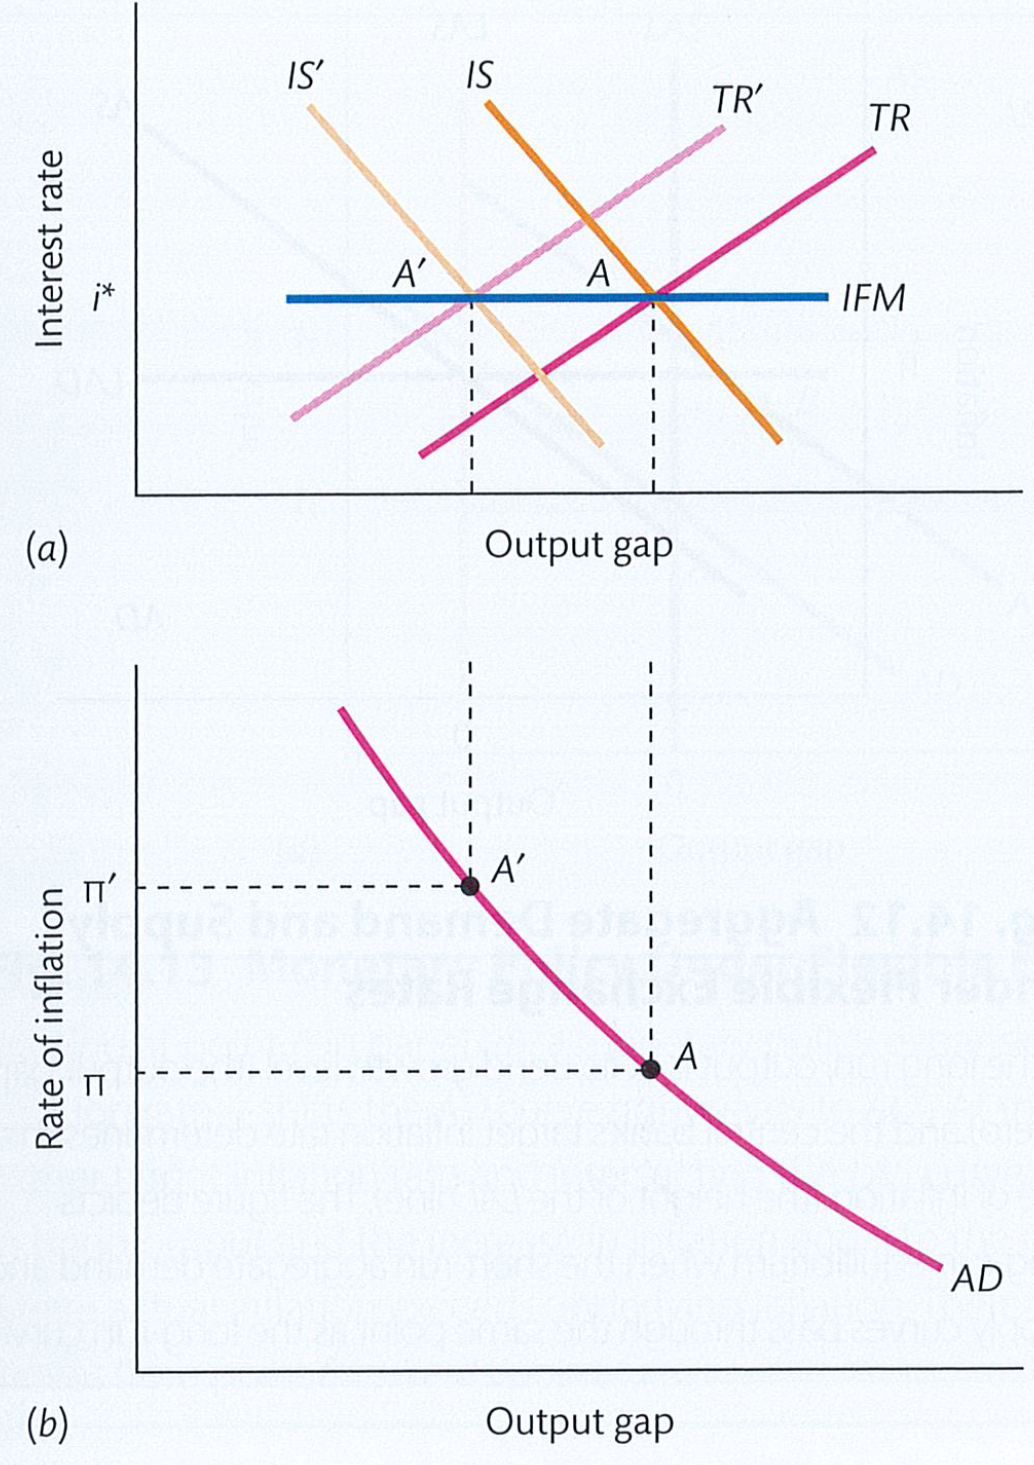
\includegraphics[clip,width=1.1\columnwidth]{FIGURES/9_ASAD_Flexible_shortrun}
%%\vspace{-2mm}
%
%\begin{minipage}{1.0\columnwidth}
%\tiny	
%%	\textbf{Note.} The Figure shows the average behaviour of variables around cyclical peaks in eight countries.\\
%\textbf{Source.} Burda and Wyplosz (2017), Figure 14.11.\\
%\end{minipage}
	
\end{columns} 	 

\end{frame}
%---FRAME------------------------------------------------------------------------------
%\subsection{How to Use the AS-AD Framework}
%---FRAME------------------------------------------------------------------------------
%\begin{frame}
%\frametitle{Outline}
%\tableofcontents[currentsubsection]
%\end{frame}
%---FRAME------------------------------------------------------------------------------
\begin{frame}{Policy example: monetary policy}
  \vspace{-3cm}
 \small \tb{Higher inflation target}, $\bar{\pi}'> \bar{\pi}$
 \vfill
%\begin{center}
%%{\footnotesize
%%Figure. Exchange rate of Danish krona vis-a-vis (a) EUR and (b) USD  \\
%%}
%%\vspace{-2mm}
%\begin{figure}[h!]
%%\caption{Figure. Net}
%	\subfigure{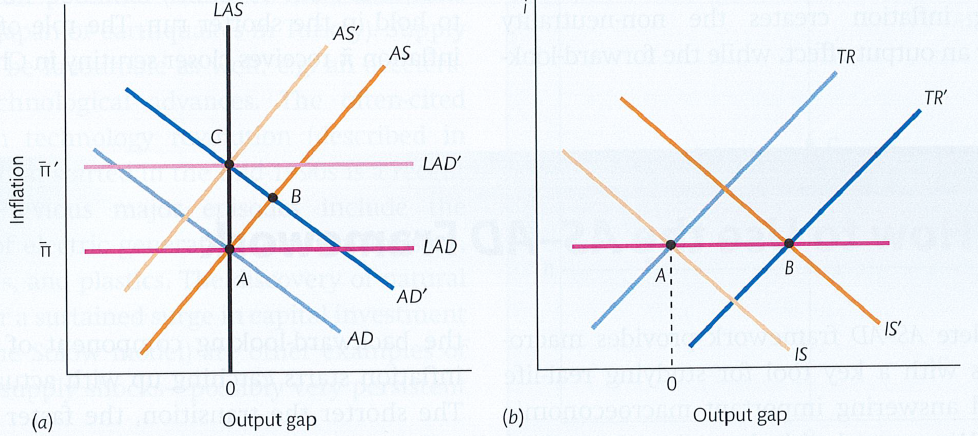
\includegraphics[trim=0 0 0 0,clip,width=0.85\textwidth]{FIGURES/9_ASAD_FlexibleMP}
%	}      
%	%} 		
%%	\label{fig:GPD} 
%	%[trim=left bottom right top
%\end{figure}
%%\vspace{-2mm}
%\begin{minipage}{0.5\columnwidth}
%\tiny	
%%\textbf{Note.} Inflation in Denmark and the euro area (1992-2016).  
%\textbf{Source.} Burda \& Wyplosz (2017), Figure 14.13.\\
%\end{minipage}
%\end{center}
\end{frame}

\begin{frame}{Policy example: government spending}
  \vspace{-3cm}
 \small \tb{Positive fiscal policy shock}, $\bar{G}'> \bar{G}$
 \vfill
\end{frame}

\section{Introduction to Dynamics: Multiplier-Accelerator}

\begin{frame}{Multiplier-Accelerator model}
  \begin{mytemize}
  \item A simple Keynesian model of the goods market 
	\item \tr{NOT} the way we think about cycles today!
  \item Motivation is methodological: look at a \tb{dynamic} equilibrium
  \end{mytemize}
  \vfill
  Three equations:
  \begin{mytemize}
  \item  Consumption depending on \textbf{last period} income
  \item  Investment depending on \textbf{growth of} income in \textbf{last period} --- the \tb{accelerator} assumption
  \item Goods market equilibrium
  \end{mytemize}
\end{frame}

\begin{frame}{Multiplier-Accelerator accelerator model}{Variables}

\begin{mytemize}
\item
  \(\{C_t\}\) --- sequence of levels of aggregate consumption
  , main endogenous variable in the model.\\
\item
  \(\{I_t\}\) --- sequence of rates of investment, another key
  endogenous variable.\\
\item
  \(\{Y_t\}\) --- sequence of levels of national income, yet another
  endogenous variable.
\item
  \(\{G_t\}\) --- sequence of levels of government expenditures. Exogenous, assumed constant: \(G_t = G\) for all \(t\).\\
\end{mytemize}

\end{frame}

\begin{frame}{Multiplier-Accelerator accelerator model}{ Model structure}

The model combines the consumption function

 \[
C_t = a Y_{t-1} + \gamma \tag{1}
\]

with the investment accelerator

 \[
I_t = b (Y_{t-1} - Y_{t-2}) \tag{2}
\]

and the goods market equilibrium

 \[
Y_t = C_t + I_t + G_t \tag{3}
\]

\begin{mytemize}
 
\item
  The parameter $a$ is people's \emph{marginal propensity to consume}
  out of income - equation
  \protect\hyperlink{equation-consumption}{(1)} asserts that people
  consume a fraction of \(a \in (0,1)\) of each additional dollar of
  income.\\
\item
  The parameter \(b > 0\) is the investment accelerator coefficient -
  equation \protect\hyperlink{equation-accelerator}{(2)} asserts that
  people invest in physical capital when income is increasing and
  disinvest when it is decreasing.
\end{mytemize}

\end{frame}

\begin{frame}{Solution: a difference equation}

  Combining the three equations:
  $$
Y_t = (a+b) Y_{t-1} - b Y_{t-2} + (\gamma + G_t)
$$
\vfill
Defining new coefficients gives compact form: assume $\rho_1 = (a+b)$ and $\rho_2 = -b$, then:
$$
Y_t = \rho_1 Y_{t-1} + \rho_2 Y_{t-2} + (\gamma + G_t) 
$$
\vfill
Assuming initial values to generate ${Y_t}$ for $ t=0, \ldots, T $:

$$
Y_{-1} = \bar Y_{-1}, \quad  Y_{-2} = \bar Y_{-2}
$$

When solving numerically, set $(a,b) $ so that starting from
$(\bar Y_{-1}, \bar Y_{-2})$,  ${Y_t}$ converges to
a \tb{steady state}

\end{frame}

\begin{frame}{A dynamic equilibrium in explicit form}
  With eigenvalues $\lambda_1, \lambda_2$, the dynamics of $Y_t$ given by:
  $$
Y_t = \lambda_1^t c_1 + \lambda_2^t c_2
$$
where $ c_1 $ and $ c_2 $ are constants on parameters and initial conditions.
initial conditions and on $ \rho_1, \rho_2 $.
\vfill
When the eigenvalues are complex, can represent them in polar form $
\lambda_1 =  r e^{i \omega}, \  \lambda_2 = r e^{-i \omega}
$ and rewrite the solution as follows (\alert{not necessary to memorize!}):
$$
  Y_t =  (c_1 + c_2) r^t \cos(\omega t) + i (c_1 - c_2) r^t \sin(\omega t)
$$
Parameters and intital conditions chosen such that $c_1+c_2$ real, $c_1-c_2$ complex, so $Y_t$ real and has a form:
$$Y_t = 2 v r^t  \cos (\omega t + \theta),$$ with $v, \theta$ some constants depending on parameters and intial conditions.
\vfill
Recall graphs of $\cos$ function \rarr output (as well as investment and consumption) oscillate around steady state.
\end{frame}



%---FRAME------------------------------------------------------------------------------
%\begin{frame}{Empirical evidence for non-neutrality?}
%
%\begin{itemize}
%\small
%\item We have split our analysis in three time horizons: \tb{short, medium and long run}. What do they mean in practice?
%\begin{itemize}
%\small
%\item \emph{Short run}: one to two years
%\item \emph{Medium run}: two to five years
%\item \emph{Long run}: beyond 5 years
%\end{itemize}
%\end{itemize}
%
%%\frametitle{Evidence of monetary policy non neutralities}
%
%\begin{center}
%{\small
%Figure. Estimated dynamic response to monetary policy shock
%}
%\end{center}
%\vspace{-2mm}
%\begin{figure}
%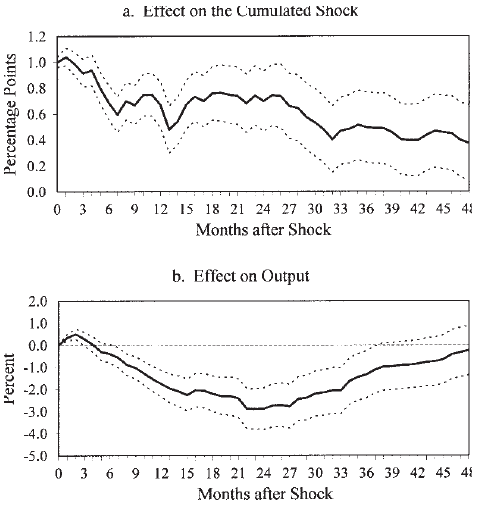
\includegraphics[width=0.4\textwidth]{FIGURES/RomerRomerFig9_ab}
%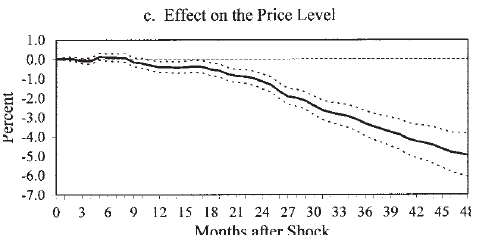
\includegraphics[width=0.4\textwidth]{FIGURES/RomerRomerFig9_c}
%\end{figure}
%\begin{minipage}{0.99\columnwidth}
%\tiny	
%\textbf{Note.} The effects of a (US) monetary policy shock in a VAR model. The authors use a narrative approach for the construction of monetary policy shocks. \emph{Source:} Romer \& Romer (2004), Figure 9.
%\end{minipage}
%
%
%\end{frame}
%%---FRAME-----------------------------------------------------
%\begin{frame}{Further evidence of monetary policy non neutrality}
%
%\begin{center}
%{\small
%Figure. Estimated dynamic response to monetary policy shock
%}
%\end{center}
%\begin{figure}
%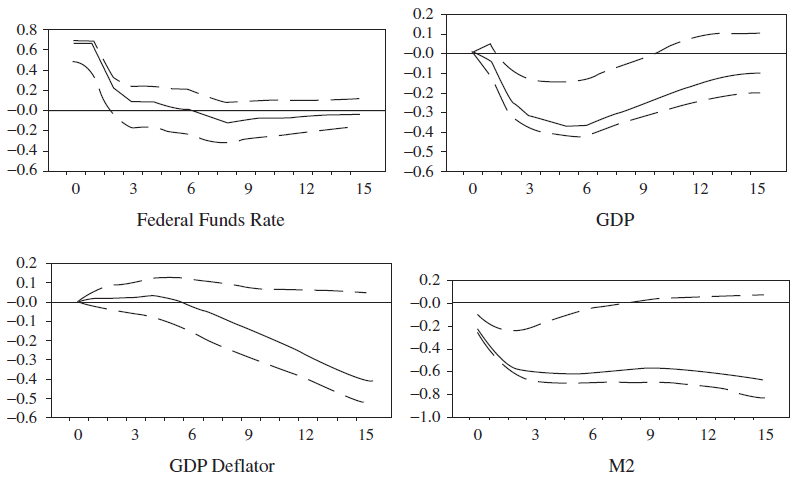
\includegraphics[width=0.75\textwidth]{FIGURES/CEE1999}
%\end{figure}
%\begin{minipage}{0.99\columnwidth}
%\tiny	
%\textbf{Notes.} The effects of a (US) monetary policy shock in a VAR model, frequency is a quarter. Depending on the identifying assumptions, the results might vary substantially. \emph{Source:} Christiano, Eichenbaum and Evans (1999), as shown in Gali (2008), Figure 1.1.
%\end{minipage}
%
%
%
%\end{frame}
%---FRAME------------------------------------------------------------------------------
\end{document}

